\documentclass[final]{siamltex}
%test change
\usepackage{cite}
\usepackage{graphicx,bbm,pstricks,soul}
\usepackage{pifont}
\usepackage{bbm,algorithmic,mdframed,placeins,multirow,booktabs,subfigure}
\usepackage[ruled,vlined,linesnumbered]{algorithm2e}
\usepackage{tikz,hhline}
\usetikzlibrary{positioning,automata}
\usetikzlibrary{arrows,fit}
\usetikzlibrary{decorations.pathmorphing}
\usepackage{tabularx}
\newcolumntype{L}[1]{>{\raggedright\let\newline\\\arraybackslash\hspace{0pt}}m{#1}}
\newcolumntype{C}[1]{>{\centering\let\newline\\\arraybackslash\hspace{0pt}}m{#1}}
\newcolumntype{R}[1]{>{\raggedleft\let\newline\\\arraybackslash\hspace{0pt}}m{#1}}

\let\oldnl\nl% Store \nl in \oldnl
\newcommand{\nonl}{\renewcommand{\nl}{\let\nl\oldnl}}% Remove line number for one line

\setlength{\parindent}{0in}
\usepackage{amsmath,amsfonts,amsbsy,amssymb}
\newcommand{\RARR}[3]{#1
  \;\displaystyle\mathop{\displaystyle\longrightarrow}^{#3}\; #2}
\newcommand{\RARRlong}[3]{#1
  \;\displaystyle\mathop{-\!\!\!-\!\!\!-\!\!\!-\!\!\!-\!\!\!\!\displaystyle
  \longrightarrow}^{#3}\; #2}
\newcommand{\LARR}[3]{#1
  \;\displaystyle\mathop{\displaystyle\longleftarrow}^{#3}\; #2}
\newcommand{\LRARR}[4]{{\mbox{ \raise 0.4 mm \hbox{$#1$}}} \;
  \mathop{\stackrel{\displaystyle\longrightarrow}\longleftarrow}^{#3}_{#4}
  \; {\mbox{\raise 0.4 mm\hbox{$#2$}}}}
\newcommand{\bX}{{\bf X}}
\newcommand{\vecx}{{\mathbf x}}
\newcommand{\vecy}{{\mathbf y}}
\newcommand{\vecz}{{\mathbf z}}
\newcommand{\vecq}{{\mathbf q}}
\newcommand{\bs}{{\mathbf s}}
\newcommand{\vecr}{{\mathbf r}}
\newcommand{\vecX}{{\mathbf X}}
\newcommand{\vecv}{{\mathbf v}}
\newcommand{\tick}{\ding{52}}
\newcommand{\cross}{\ding{54}}
\newcommand{\vecn}{{\mathbf n}}
\newcommand{\vecp}{{\mathbf p}}
\newcommand{\cT}{{\mathcal T}}
\newcommand{\dt}{{\mbox{d}t}}
\newcommand{\dx}{{\mbox{d} \vecx}}
\newcommand{\boldnu}{{\boldsymbol \nu}}
\newcommand{\er}{{\mathbb R}}
\renewcommand{\div}{{\rm div}}
\newcommand{\bnu}{{\bf \nu}}
\newcommand{\divergence}{\mathop{\mbox{div}}}
\renewcommand{\P}{\mathbb{P}}
\newcommand{\FP}{P_{\rm{FP}}}
\newcommand{\ME}{P_{\rm{ME}}}
\newcommand{\MEs}{P_{\rm{ME}_{S}}}
\newcommand{\D}{\mathcal{D}}
\newcommand{\G}{\mathcal{G}}
\newcommand{\N}{\mathcal{N}}
\newcommand{\X}{{\mathbf X}}
\newcommand{\Y}{{\mathbf Y}}
\newcommand{\W}{{\mathbf W}}
\newcommand{\data}{D}
\newcommand{\neff}{n_{\text{eff}}}
\newcommand{\E}{{\mathbb E}}
\renewcommand{\b}[1]{{\bf #1}}
\DeclareMathOperator*{\argmin}{arg\,min}
\DeclareMathOperator*{\argmax}{arg\,max}

\newcommand{\picturesAB}[6]{
\centerline{
\hskip #4
\raise #3 \hbox{\raise 0.9mm \hbox{(a)}}
\hskip #5
\epsfig{file=#1,height=#3}
\hskip #6
\raise #3 \hbox{\raise 0.9mm \hbox{(b)}}
\hskip #5
\epsfig{file=#2,height=#3}
}}
\newcommand{\picturesCD}[6]{
\centerline{
\hskip #4
\raise #3 \hbox{\raise 0.9mm \hbox{(c)}}
\hskip #5
\epsfig{file=#1,height=#3}
\hskip #6
\raise #3 \hbox{\raise 0.9mm \hbox{(d)}}
\hskip #5
\epsfig{file=#2,height=#3}
}}

\makeatletter  
\newcommand{\xleftrightarrows}[2][]{\mathrel{%  
 \raise.40ex\hbox{$  
       \ext@arrow 3095\leftarrowfill@{\phantom{#1}}{#2}$}%  
 \setbox0=\hbox{$\ext@arrow 0359\rightarrowfill@{#1}{\phantom{#2}}$}%  
 \kern-\wd0 \lower.4ex\box0}}  
 
\newcommand{\xrightleftarrows}[2][]{\mathrel{%  
 \raise.40ex\hbox{$\ext@arrow 3095\rightarrowfill@{\phantom{#1}}{#2}$}%  
 \setbox0=\hbox{$\ext@arrow 0359\leftarrowfill@{#1}{\phantom{#2}}$}%  
 \kern-\wd0 \lower.4ex\box0}}  
 
\def\leftrightarrowfill@{%
 \arrowfill@\leftarrow\relbar\rightarrow%
 }
\newcommand*{\centerfloat}{%
  \parindent \z@
  \leftskip \z@ \@plus 1fil \@minus \textwidth
  \rightskip\leftskip
  \parfillskip \z@skip}
\makeatother
\makeatother 

\newcommand\irregularcircle[2]{% radius, irregularity
  \pgfextra {\pgfmathsetmacro\len{(#1)+rand*(#2)}}
  +(0:\len pt)
  \foreach \a in {10,20,...,350}{
    \pgfextra {\pgfmathsetmacro\len{(#1)+rand*(#2)}}
    -- +(\a:\len pt)
  } -- cycle
}

\newcommand{\into}{\operatornamewithlimits{\longrightarrow}}
\newtheorem{dfn}{Definition}[section]

\newcommand{\ltri}{%
\,\resizebox{!}{0.25\baselineskip}{%
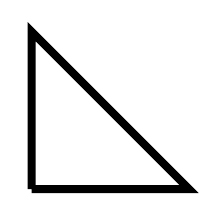
\begin{tikzpicture}%
\draw[line width=1mm](0,0) -- (0,2) -- (2,0)  -- (0,0);
\end{tikzpicture}%  
}\xspace%
}%

\newcommand{\smallltri}{%
\,\resizebox{!}{0.15\baselineskip}{%
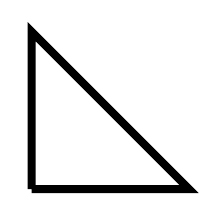
\begin{tikzpicture}%
\draw[line width=1mm](0,0) -- (0,2) -- (2,0)  -- (0,0);
\end{tikzpicture}%  
}\xspace%
}%

\title{Transport map accelerated-PAIS, and application to inverse problems arising from
  multiscale stochastic reaction networks}
\author{Simon Cotter, Yannis Kevrekidis, Paul Russell}
\begin{document}
\maketitle
\begin{abstract}
In many applications, inverse problems arise where where there are
complex correlations between the different parameters which we wish to
infer from data. The correlations often manifest themselves as lower
dimensional manifolds on which the likelihood function is
invariant, or varies very little. This can be due to trying to infer
unobservable parameters, or due to sloppiness in the model which is
being used to describe the data. In such a situation, standard
sampling methods for characterising the posterior distribution which
do not incorporate information about this structure will be highly
inefficient. Moreover, most methods are inherently serial in nature,
and as such are not expoiting the parallelised  nature of modern
computer infrastructure. In this paper, we seek to develop a method to
tackle this problem, using optimal transport maps to simplify
posterior distributions which are concentrated on lower dimensional
manifolds.

We demonstrate the approach by considering inverse problems arising
from partially observed stochastic reaction networks. In particular,
we consider systems which exhibit multiscale behaviour, but for which
only the slow variables in the system are observable. We demonstrate
that certain multiscale approximations lead to more consistent
approximations of the posterior than others.
\end{abstract}


\section{Introduction}
%Topics to cover: parallel MCMC, pMC, PAIS
%Transport maps, transport map MCMC
%Stochastic reaction networks
%Multiscale approximations, QSSA/QEA, CMA

In Section \ref{sec:map} we show how an appropriate transport map can
be constructed from importance samples which maps the posterior close
to a reference Gaussian measure. In Section \ref{sec:TPAIS} we show
how such a map can be incorporated into a sophisticated parallel MCMC
infrastructure in order to accelerate mixing. In Section
\ref{sec:multi} we consider how likelihoods can be approximated using
multiscale methodologies in order to carry out inference for
multiscale and/or partially observed stochastic reaction networks. In
Section \ref{sec:num} we present some numerical examples, which serve
to demonstrate the increased efficiency of the described sampling
methodologies, as well as investigating the posterior approximations
discussed in the previous section. We conclude with a discussion in
Section \ref{sec:conc}.

\section{Deterministic Resampling Methods}\label{sec:intro_optim}

Optimal transportation arises in many industries. It deals with the efficient allocation
of a particular resource to someone who wishes to use this resource. For example a fresh food
supplier may have many depots around the country, each with a certain number of vans capable of
carrying a fixed amount of product a particular distance in a day. The supplier may need to supply
many supermarkets up and down the country with their produce. The supplier naturally wishes to
perform this task quickly, and using as little fuel as possible. To achieve this goal the supplier
can choose which depot or depots deliver to which supermarket, and whether a van stops at zero, one
or more supermarkets on its route. The efficient solution of this problem can make a huge difference
to the profits of the supplier.

The supplier knows the initial distribution, $\mu$, where we have all of the fresh produce,
and they also know where we want it to go, the target distribution, $\eta$. We need to find a map which converts
the initial distribution, $\mu$, into the target, $\eta$. These
maps are known as transport maps. We can also contrain the problem to one where we must use as little fuel as possible, the map satisfying this condition is known as the optimal transport map.

\begin{dfn}[Transport Map~\cite{reich2013ensemble}]\label{def:transport_map}
Given a random variable $X \sim \mu$, $X \in \mathcal{X}$, and a second probability measure $\nu$, a
measurable function $T\colon \mathcal{X}\rightarrow\mathcal{X}$ is a transport map if the induced
random variable $Y = T(X)$ satisfies
\[
	\int_\mathcal{X} \! f(y)\nu(\text{d}y) = \int_\mathcal{X} \! f(T(x))\mu(\text{d}x),
\]
for all functions $f\colon \mathcal{X} \rightarrow \mathbb{R}$.
\end{dfn}

Mathematically, the formulation of this assignment problem is quite abstract. The original
formulation by Monge in 1781~\cite{monge1781memoire}, is to find the transport map, $T(\cdot)$,
which minimises the integral
\[
	\int_\mathcal{X} \! c(s, T(s)) \, \text{d}\mu(s),
\]
subject to the constraint that $T(\mu) = \nu$. We are able to choose what we consider to be
expensive by choosing the cost function $c(x,y)$ which is non-negative for all states
$x,y\in\mathcal{X}$.

A more widely used formulation of the Monge problem was presented by Kantorovitch in
1942~\cite{kantorovitch1958translocation}. This formulation considers a space of joint probability
distributions known as the space of transference plans, $\Pi(\mu, \nu)$.

\begin{dfn}[Coupling, Transference Plan~\cite{reich2013ensemble}]\label{def:coupling}
Given two distributions $\mu$ and $\nu$ on a space $\mathcal{X}$, a coupling of these distributions
is a pair $Z = (X,Y)$ such that $X\sim\mu$ and $Y\sim\nu$. The joint measure $\eta$, where
$Z\sim\eta$, on $\mathcal{Z}=\mathcal{X}\times\mathcal{X}$ is known as the transference plan for
this coupling.
\end{dfn}

The optimisation problem then becomes
\[
	\int_{\mathcal{X}\times\mathcal{X}} \! c(x, y) \, \text{d}\gamma(x, y),
\]
subject to $\gamma(x,y) \in \Pi(\mu, \nu)$. Kantorovitch also developed the field of
linear programming to help deal with solutions to this
problem~\cite{kantorovich1960mathematical,kantorovitch1958translocation}.

When the cost function is $c(x,y) = \|x - y\|^2$, if $\mu$ is absolutely continuous with respect to
Lebesgue measure, and both $\mu$ and $\nu$ have finite second order moments, then it is guaranteed
that there is a unique optimal transference plan, between $\mu$ and $\nu$~\cite{knott1984optimal}.

%%%%%%%%%%%%

\subsection{Coupling Probability Distributions}\label{sec:coupling}

In this section we return to the idea of coupling probability distributions, and motivate their use
in resampling algorithms. We defined a coupling in Definition~\ref{def:coupling} as a pair of random
variables $Z = (X,Y)$, the joint probability distribution for this pair being a quantity of
interest. In this section we assume that the marginal distributions of both $X$ and $Y$ are known,
later on we relax this so that one of these distributions is not known but can be approximated by a
sample. All distributions used in the later chapters will be absolutely continuous on $\mathcal{X} =
\mathbb{R}^n$, so we have $\mu(\text{d}x) = \pi_0(x)\text{d}x$ and $\nu(\text{d}x) =
\pi(x)\text{d}x$. Having absolutely continuous marginals does not mean that the coupling itself is
absolutely continuous.

\begin{figure}
\centering
\subfigure[$\rho = 0.1$]{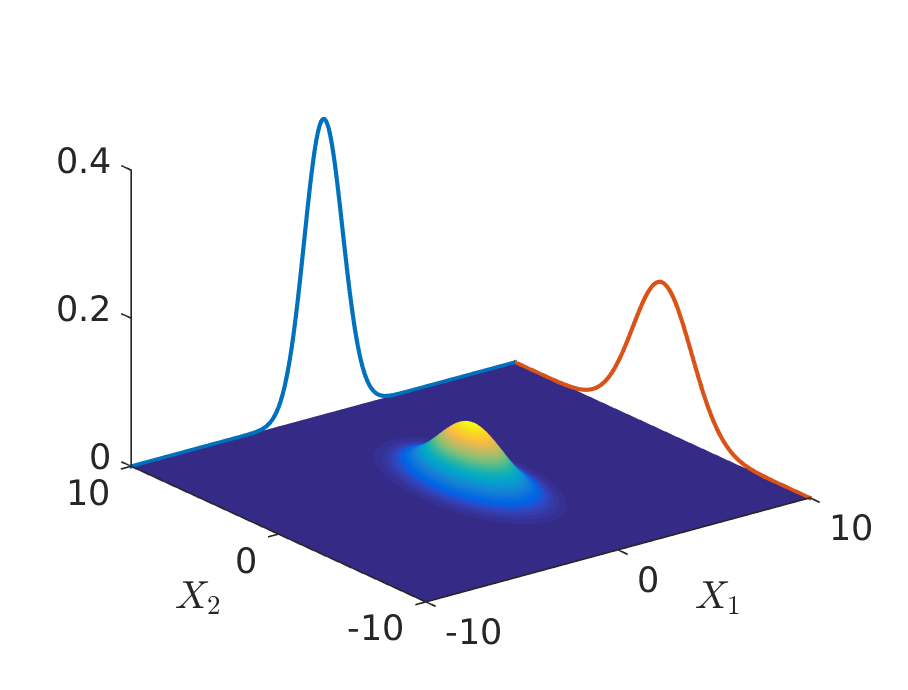
\includegraphics[width=0.45\textwidth]{images/coupling_indep}}
\subfigure[$\rho = 0.95$]{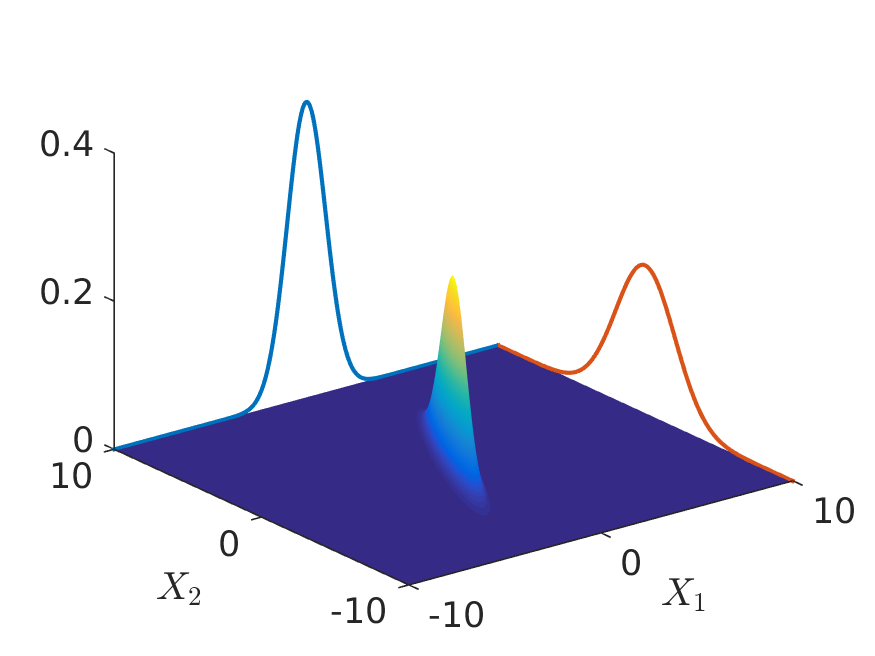
\includegraphics[width=0.45\textwidth]{images/coupling_correlated}}
\caption{Couplings with different correlations.}
\label{fig:cts_couplings}
\end{figure}

We now look at couplings between continuous random variables. As an example we consider coupling two
univariate Gaussian distributions, $X_1 \sim \mathcal{N}(\mu_1, \sigma^2_1)$ and $X_2 \sim
\mathcal{N}(\mu_2, \sigma^2_2)$. We know that the transference plan $\gamma(x_1, x_2)$ will be the
bivariate Gaussian distribution,
\[
	Z = (X_1, X_2), \quad Z \sim \mathcal{N}\left(\begin{pmatrix}\mu_1\\\mu_2\end{pmatrix},
		\begin{pmatrix} \sigma^2_1 & \rho\sigma_1\sigma_2 \\ \rho\sigma_1\sigma_2 & \sigma^2_2
		\end{pmatrix}\right).
\]
The form of this bivariate Gaussian is restricted by the marginal distributions to have this
covariance matrix, where we can choose the correlation $-1 \leq \rho \leq 1$. This unknown
correlation means that there are infinitely many couplings between $X_1$ and $X_2$, some examples
are given in Figure~\ref{fig:cts_couplings}, which leads us back to the idea of optimising the
transport map to maximise some criterion. We might want to maximise the correlation between the two
random variables. If we consider the conditional distribution $X_1|X_2 \sim \mathcal{N}(x_1; \mu,
\sigma^2)$, where
\[
	\mu = \mu_1 - \frac{\rho\sigma_1\sigma_2}{\sigma^2_2}(\mu_2 - x_2) \quad \text{and} \quad \sigma^2 =
		\sigma^2_1 - \frac{(\rho\sigma_1\sigma_2)^2}{\sigma_2^2} = (1-\rho^2)\sigma_1^2,
\]
we notice that as $\rho\rightarrow 1$ the variance $\sigma^2 \rightarrow 0$, and we obtain a
deterministic coupling with transport map $T\colon x_1 \mapsto \mu_1 -
\frac{\sigma_1}{\sigma^2}(\mu_2 - x_2)$. If we set $\mathcal{N}(\mu_2, \sigma^2_2) = \mathcal{N}(0,
1)$ we see that this coupling matches our standard map for transforming standard Gaussian random
variables into general Gaussian random variables.

Here we consider an optimal coupling to be one which maximises the correlation between $X_1$ and
$X_2$. Maximising the correlation is equivalent to minimising the expectation of $(X_2-X_1)^2$,
\[
	\mathbb{E}[(X_2-X_1)^2] = \mathbb{E}[X_1^2]+\mathbb{E}[X_2^2] - 2\mathbb{E}[X_1]\mathbb{E}[X_2]-
		2\text{cov}(X_1, X_2).
\]
The coupling which maximises the correlation is therefore the solution to the Monge-Kantorovich
problem with cost function
\[
	c(X_1,X_2) = \|X_1-X_2\|^2.
\]
This problem always has a solution since for any marginals densities $\pi_X(x)$ and $\pi_Y(y)$, the
trivial coupling $\pi_Z(x,y) = \pi_X(x)\pi_Y(y)$ exists.

We now look at couplings between two discrete random variables. Unlike in the continuous case where
the coupling had support over all of $\mathcal{X}\times\mathcal{X}$, for couplings between discrete
random variables this is rarely the case.

Consider two discrete R.V.s
\[
	Y_1 \sim \mu_{Y_1} \quad \text{and} \quad Y_2 \sim \mu_{Y_2},
\]
defined over a parameter space $\mathcal{Y} = \left\{a_1, \dots, a_M\right\}$, $a_i \in \mathbb{R}$.
Assign the mass functions
\[
	\mathbb{P}(Y_1 = a_i) = \frac{1}{M} \quad \text{and} \quad \mathbb{P}(Y_2 = a_i) = w_i,
\]
where $w_i \geq 0$ and $\sum_i \! w_i = 1$. All possible couplings $Z = (Y_1, Y_2)$ can be described
by the matrix $T \in \mathbb{R}^{M\times M}_+$, such that
\begin{equation}\label{eq:coupling_conditions}
\mathbb{P}(Y_2) = MT\mathbb{P}(Y_1), \quad \text{subject to} \quad \sum\limits_{i=1}^M \! t_{ij} =
\frac{1}{M}, \quad \sum\limits_{j=1}^M \! t_{ij} = w_i,
\end{equation}
where $[T]_{ij} = t_{ij}$.

We present two special cases, first the map with zero correlation, or trivial map,
\[
T^t = \frac{1}{M}\begin{bmatrix} w_1 & \dots & w_1 \\ \vdots & & \vdots \\ w_M & \dots & w_M
\end{bmatrix}
\]
It is clear that, after renormalisation, along any row we obtain a uniform distribution,
$\mathbb{P}(Y_1)$, and along any column we obtain the distribution $\sum_{i=1}^M
\delta_{a_i}(\cdot)w_i$, $\mathbb{P}(Y_2)$. Hence our conditionals are equal to our marginals and
there is no correlation.

The second case is more interesting. The coupling which maximises the correlation between the two
marginals, $T^*$, is the solution to the optimisation problem
\[
	T^*  = \arg\min_T \! \sum\limits_{i,j=1}^M \! t_{ij}(a_i - a_j)^2,
\]
subject to the row and column constraints on $T$ in Equation~\eqref{eq:coupling_conditions}~\cite{reich2015probabilistic}.

We now look at a simple example of a discrete coupling. Given a state space $\mathcal{Y} = \{a_1,
\dots, a_M\}$ where $M=5$, and two probability distributions defined over $\mathcal{Y}$,
\[
\mathbb{P}(Y_1 = a_i) = \frac{1}{M} \quad \text{and} \quad \mathbb{P}(Y_2 = \mathbf{a}) = (0.1,
0.25, 0.05, 0.3, 0.3)^\top.
\]
If we assume that the states $a_i$ are sorted so that $a_i < a_{i+1}$ for all $i=1,\dots,M-1$, then
the optimal coupling is
\[
	T^* = \begin{bmatrix} 0.1 & 0      & 0    & 0    & 0 \\
					       0.1 & 0.15 & 0    & 0    & 0 \\
					       0    & 0.05 & 0    & 0    & 0 \\
					       0    & 0      & 0.2 & 0.1 & 0 \\
					       0    & 0      & 0    & 0.1 & 0.2
		\end{bmatrix}.
\]
For an ordered state space we can construct this coupling following this staircase pattern by
starting in the top left and filling first the row then the column heading towards the bottom right
corner. We notice that this staircase structure corresponds to the shape seen in the highly
correlated coupling in Figure~\ref{fig:cts_couplings} (b). The $2M-1$ constraints mean that we have
at most $2M-1$ non-zero entries, so the support of the joint distribution is much smaller than the
full space.

The product $MT^*$ results in a column stochastic matrix $P$. If we want to draw an evenly weighted
sample, $\{s_i\}_{i=1}^5$, which obeys the probability law $\mathbb{P}(Y_2)$, we can use the columns
of $P$ as probability distributions,
\[
	s_1 \sim \frac{1}{2}\delta_{a_1}(\cdot)+\frac{1}{2}\delta_{a_2}(\cdot), \quad s_2 \sim
		\frac{3}{4}\delta_{a_2}(\cdot)+\frac{1}{4}\delta_{a_3}(\cdot), \quad s_4 \sim
		\frac{1}{2}\delta_{a_4}(\cdot)+\frac{1}{2}\delta_{a_5}(\cdot),
\]
and deterministically $s_3 = a_4$, $s_5 = a_5$. What we have done here is used an optimal coupling
between weighted and unweighted random variables to resample from the weighted distribution.

%%%%%%%%%%%%

\subsection{Resampling with Filters}
\label{sec:OT}

Resampling is a method which is distinct from most of the Statistical literature in that rather than
sampling from a known parametric distribution which is usually the aim, we instead attempt to sample
from empirical distributions. These distributions often arise from a sample, $\{(w_i,
\theta_i)\}_{i=1}^n$, in the form,
\begin{equation}\label{eq:empirical_dist}
\pi(\cdot) = \sum\limits_{i=1}^n \! w_i\delta_{\theta_i}(\cdot), \quad \text{where}
\quad\sum\limits_{i=1}^n \! w_i = 1.
\end{equation}
The weights, $w_i$ may be equal to $1/n$ or they may all be different.
\begin{dfn}[Resampling]\label{def:resampling}
Given a discrete empirical distribution of the type in Equation~\eqref{eq:empirical_dist}. Resampling provides
us a new discrete distribution of the form
\[
	\tilde{\pi}(\cdot) = \frac{1}{n}\sum\limits_{i=1}^n \! n_i\delta_{\theta_i}(\cdot), \quad
		\text{where} \quad n_i \in \{0,\dots,n\}, \quad \sum\limits_{i=1}^n \! n_i = n.
\]
The density $\tilde{\pi}$ is in some way close to the original density $\pi$.
\end{dfn}
In Definition~\ref{def:resampling} the condition on the sum of the $n_i$ restricts $\tilde{\pi}$ to
be composed of the same number of samples as $\pi$. This is not necessary although as mentioned in
Section~\ref{sec:gmh} one can run into trouble when this is not the case. These problems arise
because the empirical density $\pi$ is usually approximating some continuous distribution, $f$, and
over reliance on one approximation will cause the tails of the $f$ to be underestimated. If a sample
is required, one uses $n_i$ lots of $\theta_i$, otherwise statistics can be computed directly from
$\tilde{\pi}$.

%%%%%%

\subsubsection{Bootstrap Resampling}

One of the first resamplers capable of accomplishing the feat in Definition~\ref{def:resampling} was
the bootstrap resampler (BSR)~\cite{efron1992bootstrap}.

\begin{table}[htpb]
\begin{algorithm}[H]
\DontPrintSemicolon
\BlankLine
Obtain sample, $\{x_i\}_{i=1}^n$ from some distribution.\;
Construct
\[
	\hat{F} = \sum\limits_{i=1}^n \! n_i\delta_{x_i}(\cdot), \quad n_i = \sum\limits_{k=1}^n \!
		\text{I}(x_i = x_k).
\]

Sample with replacement $X^* = [x^*_1,\dots,x_n^*]^\top \sim \hat{F}$. i.e. $X^* \sim
\text{Multi}(1, \frac{1}{n}[n_1,\dots,n_n]^\top)$.\;
\caption{The Bootstrap Resampler~\cite{efron1992bootstrap}.\label{alg:bs_resampler}}
\end{algorithm}
\end{table}

Algorithm~\ref{alg:bs_resampler} presents the BSR when we have an evenly weighted sample, this can
just as easily be extended to a weighted sample, $\{(w_i, x_i)\}_{i=1}^n$. In this case the
probability vector in the Multinomial distribution becomes $\tilde{\mathbf{w}} = [\tilde{w}_1,
\dots, \tilde{w}_n]^\top$ where $\tilde{w}_i = \sum_{k=1}^n \! w_i\text{I}(x_i = x_k)$.

%%%%%%

\subsubsection{The Bootstrap Particle Filter}

The data assimilation community is concerned with predicting the state of time dependent systems
given noisy observations. This type of problem is known as the filtering problem. Usually there is a
model for the system although it may be expensive to evaluate. We assume that we have a prediction,
$x(t)=[x_1(t),\dots,x_N(t)]^\top$, from the model calculated using observations, $D_i(t-1)$. We also
observe some data at time $t$, $D_i(t)$. An application of Bayes' formula allows us to combine these
two pieces of information to refine the prediction.
\begin{dfn}[Particle Filter]
A particle filter is an algorithm which solves the filtering problem.
\end{dfn}

\begin{table}[htpb]
\begin{algorithm}[H]
\DontPrintSemicolon
\BlankLine
Define a system model,
\[
	x_i(t) = f_{t-1}(x_i(t-1), \xi_i(t-1)), \quad \text{where} \quad f_t\colon
		\mathbb{R}^n\times\mathbb{R}^m\rightarrow\mathbb{R}^n, \quad \xi_i(t-1) \sim \mathcal{N}(0,
\sigma^2).
\]

\nonl \textbf{Predict}\;
Sample $\xi_i(t-1) \sim \mathcal{N}(0, \sigma^2)$.\;
Calculate $x_i^*(t) = f_{t-1}(x_i(t-1), \xi_i(t-1))$.\;
\nonl\;
\nonl \textbf{Update}\;
For each particle calculate
\[
	w_i = \frac{\ell(D_i(t)| x_i^*(t))}{\sum_{k=1}^N \! \ell(D_k(t)| x_k^*(t))}.
\]

Resample $x(t) \sim \text{Multi}(1, w/\|w\|_1)$, where $w = (w_1,\dots,w_N)^\top$.
\caption{The Bootstrap Particle Filter~\cite{gordon1993novel}.\label{alg:bs_filter}}
\end{algorithm}
\end{table}
The bootstrap filter is an early particle filter, consisting of two steps. The first is to propogate
the prior's predictions through the system model. We then assign a weight to each particle based on
how likely the data we have just received is given the prior prediction. Finally we use the
bootstrap resampler to convert these weighted particles into the estimate of the current state. This
current state can become the prior information for the next iteration.

%%%%%%

\subsubsection{Linear Ensemble Transform Filters}

The bootstrap filter is a random transformation of the empirical density, $\pi$, and the transformed
density, $\tilde{\pi}$, has the same support as $\pi$, with a number of copies of each
particle. It is often undesirable for us to have copies since this means that we do not cover as
much of the sample space as we could. This leads to wasted computation, poorer quality samples and a
worse approximation of the densities of interest. One method of reducing the number of repeats in a
sample is to allow $\tilde{\pi}$ to be built from linear combinations of the original sample. This
means that the support of the density $\tilde{\pi}$ is not restricted to being the same as $\pi$ and
reduces the likelihood of having two particles in the same position. Particle filters which use
linear combinations to produce the transformed density are known as Linear Ensemble Transform
Filters (LETFs).

\begin{dfn}[Linear Ensemble Transform Filter]\label{def:LETF}
A particle filter where the original sample, $\{\theta_i\}_{i=1}^M$, is transformed into a new
sample, $\{\tilde{\theta}_i\}_{i=1}^M$, according to the relation
\[
	\tilde{\theta}_j = \sum\limits_{i=1}^M \! w_{ij}\theta_i, \quad w_{ij} \geq 0, \ \sum\limits_{i=1}^M
		w_{ij} = 1,
\]
is known as a linear ensemble transform filter.
\end{dfn}

%%%%%%

\subsubsection{The Ensemble Transform Particle Filter}

The ensemble transform particle filter (ETPF) proposed by Reich in~\cite{reich2013nonparametric} is
an ensemble transform method which combines the optimal coupling ideas from
Section~\ref{sec:coupling} with the LETF framework to produce a particle filter which is consistent
in the limit of the ensemble size $M\rightarrow\infty$. The transform takes a sample of weighted
particles $\{(w_i,y_i)\}_{i=1}^M$ with law$(\mu_Y) = \pi_{Y}$ and converts it into a sample of
evenly weighted particles $\{x_i\}_{i=1}^M$ with law$(\mu_{X}) = \pi_{X}$, by means of defining a
coupling $T^*$ between the distributions $Y$ and $X$. The couplings used here are optimal in the
sense discussed in Section~\ref{sec:coupling}. The coupling $T^*$ is the solution to a linear
programming problem in $M^2$ variables with $2M-1$ constraints as defined in
\cite{reich2013nonparametric}. Choosing to maximise the correlation means that a statistic $s(X)
\rightarrow s(Y)$ as $M\rightarrow\infty$, and $s(X)$ converges faster than any other random
variable induced by a linear coupling. The density $\pi_X$ is the optimal density for approximating
$\pi_Y$ given that the mixture components have equal variance and equal weight.

\begin{table}[htpb]
\begin{algorithm}[H]
\DontPrintSemicolon
\BlankLine

\nonl \textbf{Predict}\;
Sample $\xi_i(t-1) \sim \mathcal{N}(0, \sigma^2)$.\;
Calculate $x_i^*(t) = f_{t-1}(x_i(t-1), \xi_i(t-1))$.\;
\nonl \textbf{Update}\;
For each particle calculate
\[
	w_i = \frac{\ell(D_i(t)| x_i^*(t))}{\sum_{k=1}^N \! \ell(D_k(t)| x_k^*(t))}.
\]

Find the optimal coupling,
\[
	T^* = \arg\min\limits_{T} \sum\limits_{i,j=1}^M \! t_{ij}\|x_i^*(t) - x_j^*(t)\|^2_2.
\]

Set $x(t) = M(T^*)^\top x^*(t)$.\;

\caption{The Ensemble Transform Particle Filter~\cite{reich2013nonparametric}.\label{alg:ETPF}}
\end{algorithm}
\end{table}

The ETPF is outlined in Algorithm~\ref{alg:ETPF}. It follows the same structure as the bootstrap
filter in Algorithm~\ref{alg:bs_filter}, but in this case the resampling step is performed by taking
a linear combination of the prior states rather than sampling from a multinomial distribution. The
conditions on the $t_{ij}$ are given in Equation~\eqref{eq:coupling_conditions}.

%%%%%%

\subsubsection{Approximate Multinomial Resampling}

The ETPF described in the previous section is optimal in terms of maximising the correlation between
the two marginal distributions. However the linear programming problem which must be solved for
every new empirical distribution is very costly, especially as the ensemble size grows. For the
purposes we require, discussed in Chapter~\ref{sec:PAIS}, we do not need as much accuracy as is
provided by the ETPF. For this reason we introduce a new algorithm, the approximate multinomial
resampler (AMR)~\cite{cotter2015parallel}, which shares many properties with the ETPF, but relaxes the constraint on
finding the optimal coupling. Instead we find a coupling via a greedy method in which the
correlation is high near particles with large weights, but is poor for particles with a low weight.

To perform the resampling, we split the state space into $M$, not necessarily disjoint subspaces,
$R_i\neq\emptyset$, each subspace containing at least one of the original samples $\{x_i\}$. We
define $M$ new probability distributions, $p^i$, such that $\sum_{i=1}^M \! p^i = w$, where $w$ is
the vector of the original probabilities corresponding to $x$. These probability distributions each
satisfy the conditions
\[
	\tilde{p}_k^i \leq w_k, \quad \|\tilde{p}^i\|_1 = \frac{1}{M},\quad \text{and}\quad p^i =
		M\tilde{p}^i.
\]
At this point, we could still be talking about the ETPF. The distinction comes in the way that we
choose the $R_i$ and $\tilde{p}^i_k$. We choose to first pick the particle, $x_J$, with the highest
weight and then expand a ball around it until the ball contains $1/M$ of the total probability mass.
The particle furthest from $x_J$ inside the ball may have its weight reduced by the amount required
for $\|\tilde{p}^i\|_1=1$. All other particles in the ball will have $\tilde{p}^i_k = w_k$. Once
this is done, particles which have had all their probability mass assigned to a distribution $p^i$
are removed, and we choose the particle with the next highest weight.

This method ensures that areas with a high weight have a particle chosen in that area again. The
greedy nature of the algorithm means that the correlation is sub optimal. In Algorithm~\ref{alg:AMR}
we present the pseudo-code form of this algorithm.

\begin{table}[htpb]
\begin{algorithm}[H]
\DontPrintSemicolon
\BlankLine

Obtain a weighted sample $\{(w_i, y_i)\}_{i=1}^M$.\;
\For{$i=1,\dots,M$}{
	$J = \arg\max_j \! w_j$.\;
	$p_{J,i} = 1/M \wedge w_J$.\;
	$w_J = w_J - p_{J,i}$.\;
	\While{$\sum_j p_{j,i} < 1/M$}{
		$K = \arg\min_{k\in\{k|w_k>0\}} \! \|y_J - y_k\|$.\;
		$p_{K,i} = (1/M-\sum_j \! p_{j,i}) \wedge w_K$.\;
		$w_K = W_K - p_{K,i}$.\;
	}
}
$x = MP^\top y$.\label{algline:amr_mean}\;
\caption{The Approximate Multinomial Resampler~\cite{cotter2015parallel}.\label{alg:AMR}}
\end{algorithm}
\end{table}

In Line~\ref{algline:amr_mean} of Algorithm~\ref{alg:AMR} we see that the output of the algorithm,
an evenly weighted sample, takes the form required by Definition~\ref{def:LETF} to be an LETF. We
note that the AMR algorithm, like the ETPF algorithm preserves the mean of the sample,
\[
	\hat{\mu}_X = \frac{1}{M}\sum_i \! x_i = \frac{1}{M}\sum_i \sum_k \! p_{k,i}y_k = \frac{1}{M}\sum_k
		w_ky_k = \hat{\mu}_Y.
\]
Here we use that the columns of $P$ are the probability distributions $p^i$, and the sum of these
distributions is equal to the weights, $w$, hence
\[
	\sum_i \! p_{k,i}y_k = (p^1_k + \dots + p^M_k)y_k = w_ky_k.
\]

%%%%%%

\subsubsection{Numerical Comparison of the Filter Resamplers}

We have designed the AMR with the aims of being numerically cheaper than the ETPF, and more accurate
than the BSR. Therefore we now present numerical examples which demonstrate that we have achieved
this. To compare the algorithms, we write a simple MC algorithm which compares the ability of each
algorithm to preserve the statistics of a weighted sample in an evenly weighted sample.

\begin{table}[htpb]
\begin{algorithm}[H]
\DontPrintSemicolon
\BlankLine
\For{$k=1,2,\ldots,\frac{N}{M}$}{
	Sample $y_j \sim Q$, for $j = 1, \ldots, M$.\;
	Weight $y_j$ under $F$,
	\[
		w_j = F(y_j) / Q(y_j).
	\]

	Resample 
	\[
		\hat{F}_k = \sum_j w_j\delta_{y_j}(\cdot) \rightarrow \sum_j n_j\delta_{x_j}(\cdot) = \hat{G}_k \approx \hat{F}_k.
	\]

	Calculate error in the statistic
	\[
		s_k = \frac{|s(\{x_j\}) - s(\{(w_j, y_j)\})|}{|s(\{x_j\})|}.
	\]
}
Return mean($\{s_k\}$).\;
\caption{Comparing Resamplers.\label{alg:ETMC}}
\end{algorithm}
\end{table}

In Algorithm~\ref{alg:ETMC} we create random empirical weighted distributions, $\hat{F}$, which are an
approximation of a chosen distribution $F$. We then resample from $\hat{F}$ to create a new
distribution $\hat{G}$. The new empirical distribution, $\hat{G}$, follows roughly the same
distribution but some error is introduced since we require an integer number,
$n_j$, of each particle. We want to calculate how big the error is between the distributions of $\hat{F}$ and
$\hat{G}$. To do this we calculate some chosen statistics of both $\hat{F}$ and $\hat{G}$ and
calculate the relative difference between these statistics. This is done for each resampler with a fixed total sample size of $N$,
and we vary $M$ to see how the relative error varies with the ensemble sizes.

\begin{figure}[htb]
\centering
\subfigure[Relative error in $\mathbb{E}(X)$]{\includegraphics[width=0.45\textwidth]{"images/AMR_EX"}}
\subfigure[Relative error in
$\mathbb{E}(X^2)$]{\includegraphics[width=0.45\textwidth]{"images/AMR_EX2"}}\\
\subfigure[Relative error in $\mathbb{E}(X^3)$]{\includegraphics[width=0.45\textwidth]{"images/AMR_EX3"}}
\subfigure[Cost of resamplers per iteration]{\includegraphics[width=0.45\textwidth]{"images/AMR_speed"}}\\
\caption{Relative errors representing the error between $\hat{F}$ and $\hat{G}$ as described in Algorithm~\ref{alg:ETMC}, where $\hat{G}$ is constructed using the Bootstrap, ETPF and AMR algorithms.}
\label{fig:AMR}
\end{figure}

To test the resamplers we chose a proposal distribution, $Q = \mathcal{N}(1,2)$, and a target
distribution $F = \mathcal{N}(2,3)$. Figure \ref{fig:AMR} (a)-(c) shows how the relative errors in
the first three raw moments varies with ensemble size $M$. As expected, the AMR lies somewhere
between the high accuracy of the ETPF and the less accurate BSR. Note that only the error for the
BSR is presented for the first moment since both the ETPF and the AMR are mean preserving. Figure
\ref{fig:AMR} (d) shows how the computational cost, measured in seconds, scales with the ensemble
size. These results demonstrate that the AMR behaves how we wish, and importantly ensures that
exactly one sample of the output will lie in each region with higher than average density.

%%%%%%

\subsubsection{Scaling of Resampling Algorithms with Dimension}
Ideally the dimension of particles in a filter will not affect the convergence of the method.
Unfortunately, the approximation of continuous density functions is computationally infeasible in
high dimensions with the ensemble size required to achieve convergence growing exponentially in the
dimension\cite{silverman1986density,snyder2008obstacles}.

\begin{figure}[htb]
\begin{center}
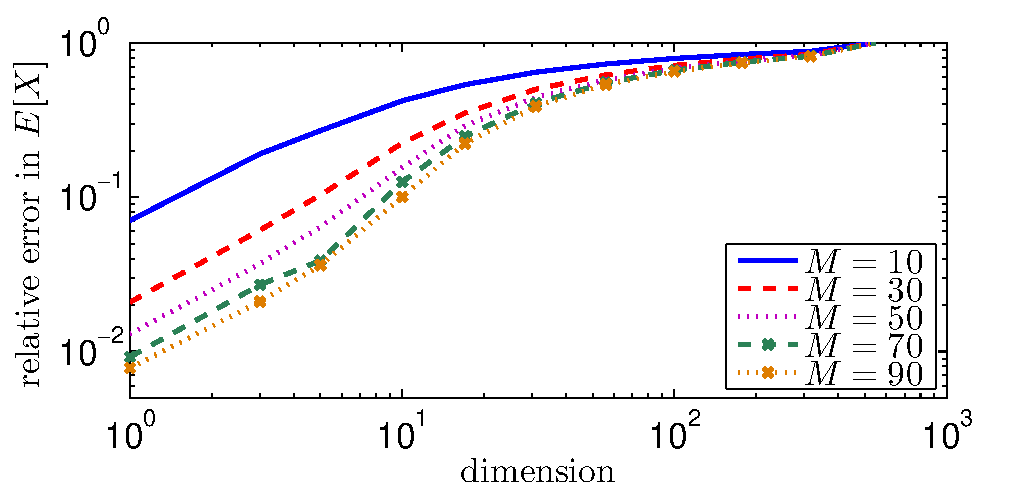
\includegraphics[width=0.7\textwidth]{images/ET_dim_scaling}
\caption{Demonstration of the ETMC algorithm rapidly failing as the dimension increases in problem
$G_1$ defined in Chapter~\ref{sec:PAIS}. The relative error shown is that between $\mathbb{E}_{\hat{F}}[X]$ and $\mathbb{E}_{\hat{G}}[X]$.}
\label{fig:ET_dim_scaling}
\end{center}
\end{figure}

Figure~\ref{fig:ET_dim_scaling} shows how quickly the ETMC algorithm loses its ability to accurately
represent the mean of the target distribution as the dimension increases. Clearly for a simple
Gaussian problem, we can not resample in much more than 10 dimensions and hope to recover a
representative sample without massively increasing the ensemble size. This phenomenon is known as
the curse of dimensionality. The AMR and BSR suffer in a similar manner as the dimension increases.

%%%%%%%%%%%%

\subsection{Couplings between Arbitrary Probability Measures}\label{sec:intro_TM}

In the previous sections we have looked at couplings which convert a weighted sample into an
unweighted sample while preserving the approximate empirical distribution. In this section we look at
how we can couple two arbitrary measures. In the following discussion we concentrate on designing a
coupling which maps from an arbitrary probability distribution onto a standard Gaussian
distribution. The main difference here is that we would like to construct a map between the
continuous distribution $F$ and a \emph{reference measure}, $\mathcal{N}(0, \text{I})$, rather than
between the approximation of $F$, $\hat{F}$, and the approximation of $\hat{F}$, $\hat{G}$.

Obviously constructing an exact map for arbitrary $F$ is infeasible, so we must again use an
empirical distribution $\hat{F}$ where $\hat{F}\rightarrow F$ in the limit of infinite samples,
however we can ensure that we are coupling $\hat{F}$ to the continuous distribution $\mathcal{N}(0,
1)$. This convergence must be achieved by continual sampling from $F$, which for an arbitrary
distribution can be expensive. To speed up this process~\cite{parno2014transport} proposes an MCMC
algorithm which sequentially updates the distribution $\hat{F}$ and recalculates the map so that
after each update, sampling from $F$ becomes cheaper. Calculating the transport map between
$\hat{F}$ and $\mathcal{N}(0, \text{I})$ allows us to sample more efficiently because it reduces the
sampling problem to sampling from a standard Gaussian distribution and then mapping these Gaussian
random variables onto an arbitrary probability measure. Which for the class of maps considered is
very cheap. These couplings are discussed further in Chapter~\ref{sec:map}.

\section{Construction of transport maps in importance sampling} \label{sec:map}
%Follow the other papers, show adaptation(s)

So far we have seen that the PAIS algorithm is efficient for low dimensional posterior sampling.
PAIS is particularly useful if the posterior is multimodal, or inconveniently shaped such as the
Rosenbrock density discussed in Chapter~\ref{chapter:HMC}. However, we have had trouble when
attempting to increase the dimension of the parameter space. This was seen when we attempted to
recover the initial condition for the wave equation in Chapter~\ref{sec:PAIS}.

In this Chapter we look at a method which will allow us to improve efficiency in low dimensions, and
will also allow us to sample more efficiently in higher dimensions. The ideal sampling
situation in MCMC is to explore an $n$-dimensional Gaussian distribution (or other standard distribution) using a near proportional
proposal distribution. We therefore aim to transform an arbitrary distribution, $\mu_\theta$, in to a Gaussian distribution, which we can then sample from efficiently, and finally transform this sample back into a sample from $\mu_\theta$. In this way we hope to be able to sample from any distribution $\mu_\theta$ with a similar efficiency as we obtain when sampling from a Gaussian distribution. In particular for the PAIS algorithm, resampling schemes are more efficient in higher
dimensions if the dimensions are uncorrelated. The work of Moselhy and
Marzouk~\cite{el2012bayesian}, Parno and Marzouk~\cite{parno2014transport} and
Parno~\cite{parno2015transport} provides a method of constructing such a map as part of an adaptive
Metropolis-Hastings algorithm.

%Given some constraints it is computationally tractable to adaptively construct invertible maps
%during an MCMC simulation. These maps construct a continuous coupling between a target and
%reference distribution, where the latter is chosen to be a standardised Gaussian. How close this reference
%distribution is to Gaussian depends on three considerations; firstly the constraints applied. These
%constraints, discussed later, ensure that the map exists, is unique, and is invertible. The
%necessity for the map to be invertible, and preferrably easily invertible, restricts the space of
%possible couplings to the point where it is unlikely that the exact map is included in our space of
%feasible transference plans. Secondly, for our purposes, the map takes the form of a polynomial
%chaos expansion which requires infinitely many terms to exactly represent the coupling. This is of course not possible on current hardware. Finally we
%will be constructing this map using an optimisation problem where the objective function depends on
%the sample path of our MCMC algorithm. This sample does not represent the target exactly until $N\rightarrow\infty$, and so the expectation is only calculated approximately.
%
%While the restrictions on the map are essential for well-posedness, the approximate map which
%results from these constraints can be made arbitrarily accurate by increasing the number of basis
%functions used in the expansion, and increasing the number of samples used in the optimisation
%problem. In practise it appears that we need not aim to achieve a high accuracy solution. Excellent
%results have been observed using monomial basis functions of total order 3, and we need a sample of
%size of only $\mathcal{O}(10^3)$ to obtain a well converged map.

In~\cite{el2012bayesian} the transport map was introduced to provide a transformation from the prior
distribution to the posterior distribution, the idea being that one could draw a moderately sized
sample from the prior distribution and use this sample to approximate a map onto the target space.
Once this map was known to the desired accuracy a larger sample from the prior could be used to
investigate the posterior distribution. This
methodology was adapted in~\cite{parno2014transport} to form a new proposal method for MH
algorithms. In this case, rather than transforming a sample from the prior into a sample from the target
distribution, the map transforms a sample from the posterior onto a reference space.
The reference density is chosen to allow efficient proposals using a simple proposal
distribution such as a Gaussian centred at the previous state. Proposed states can then be mapped back into a sample from the posterior by applying the inverse of the transport map.

Proposing new states in this way allows us to make large steps around complex probability distributions.
It is also feasible in this framework to assume that the reference density is close enough to a standard Gaussian that we can efficiently propose moves using a proposal distribution which is independent of the current state, e.g. choose $q(\theta) = \mathcal{N}(0,I_n)$.

In this chapter we introduce the derivation of the map discussed, show how it can be adapted to work
with a weighted sample, and that mixture distributions as used in the PAIS algorithm can more
efficiently approximate the reference space and so lead to higher overall effective sample sizes.
Further we show that the algorithm arising from the combination of these methods can lead to more
efficient sampling than either can achieve on its own.

\subsection{The Transport Map}

In this section we outline the methodology in \cite{parno2014transport} for coupling the target,
$\mu_{\theta}$, with the reference distribution, $\mu_r$.
We also show how the map can be constructed using a weighted sample and hence how we can incorporate the map into the PAIS algorithm.

\begin{dfn}[Transport Map $T$]
	Given a probability distribution $\mu_\theta$ with support $\mathcal{X}$.
	A transport map is a function $T\colon \mathcal{X} \rightarrow \mathbb{R}^d$ such that
	\[
		\mu_\theta(A) = \mu_r(T(A)) \quad \text{for any } A \subset \mathcal{X}.
	\]
\end{dfn}

\begin{dfn}[Exact Transport Map $T$]
	A transport map $T$ is exact if the {\it pullback} of the standard Gaussian density,
	\begin{equation}\label{eq:pullback}
		\tilde{\pi}(\theta) = \phi(T(\theta))|J_T(\theta)|,
	\end{equation}
	is equal to the target density $\pi(\theta)$ for all $\theta \in \mathcal{X}$.
\end{dfn}

In the rare case that we have the exact map, $T\in\mathcal{T}$ where $\mathcal{T}$ is the space of all invertible maps, we are able to draw a sample from $\pi_r = \phi$, the density of the standardised Gaussian distribution, and map these samples back onto target space using $T^{-1}$. These proposed samples are distributed according to the target distribution.

On target space, the proposal density is induced by the pullback of $\phi$ through $T^{-1}$.
Clearly the pullback only exists when $T$ is monotonic and has continuous first derivatives.
Not all maps satisfy these conditions, so we define a smaller space of maps, $\mathcal{T}^\uparrow \subset \mathcal{T}$ which contains all feasible maps.
The exact map $T$ is not necessarily in $\mathcal{T}^\uparrow$, so we are motivated to formulate an optimisation problem as discussed in Section~\ref{sec:intro_optim}.

We attempt to find a deterministic coupling of two continuous probability distributions, $(\mu_\theta, \mu_r)$, such that $\mu_r = T\mu_\theta$ is satisfied and also that $T \in \mathcal{T}^\uparrow$. There may be infinitely many such couplings, so we look to find the coupling which minimises the KL-divergence between the density of $\mu_{\theta}$ and the pullback of the density of $\mu_{r}$, i.e. the distance between $\pi(\theta)$ and $\tilde{\pi}(\theta)$.

When we optimise the cost function
\[
	C(T) = D_\text{KL}(\pi\|\tilde{\pi}),
\]
numerically, it is not guaranteed that the resulting map will be invertible, so it must be enforced in the design of each map component. To ensure invertibility we restrict the map to be lower triangular, i.e. $\tilde{T} \in \mathcal{T}^{\ltri}\subset\mathcal{T}^\uparrow$. This lower triangular map has the form,
\[
	T(\theta_1, \dots, \theta_n) = \begin{bmatrix} T_1(\theta_1) \\ T_2(\theta_1, \theta_2) \\ \vdots \\
		T_n(\theta_1, \dots, \theta_n) \end{bmatrix},
\]
where $T_i\colon \mathbb{R}^i \to \mathbb{R}$. We assume that the target and reference probability densities are absolutely continuous on
$\mathbb{R}^d$. Under this formulation we are guaranteed a unique invertible map $\tilde{T}$ with the property that
\[
	\mu_{\theta} \approx \tilde{T}\mu_r.
\]
Relaxing the equality constraint to; finding the approximate map $\tilde{T} \in \mathcal{T}^{\ltri}$ which minimises the distance, allows us to formulate an efficient sampling method in terms of the linear algebra required, and experimentation has shown that the departure of the reference space from Gaussian is not too severe.

\subsubsection{The optimisation problem}

With these constraints in mind we formulate the optimisation problem explicitly. The cost function
is chosen to be the Kullback-Leibler divergence between the posterior density and the pullback density,
\[
	D_\text{KL}(\pi\|\tilde{\pi}) =
		\mathbb{E}_\pi\left[\log\left(\frac{\pi(\theta)}{\tilde{\pi}(\theta)}\right)\right].
\]
Given the form of the pullback in Equation~\eqref{eq:pullback}, now taken through an approximate map, the divergence becomes
\[
	D_\text{KL}(\pi\|\tilde{\pi}) = \mathbb{E}_\pi\left[\log\pi(\theta) - \log\pi_r(\tilde{T}(\theta)) -
		\log\left|J_{\tilde{T}}(\theta)\right|\right].
\]
We note the posterior density is constant in $\tilde{T}$, and so it is not necessary for us to compute it when optimising this cost function. This expression is a complicated integral with respect to the target distribution, for which the normalisation constant is unknown, however this is exactly the scenario for which we would turn to MCMC methods for a solution.

To find the best coupling, $\tilde{T} \in \mathcal{T}^{\ltri}$, we solve the optimisation problem,
\[
	\tilde{T} = \arg\min_{T \in \mathcal{T}^{\smallltri}} \mathbb{E}_\pi\left[-\log\pi_r(T(\theta)) -
		\log\left|J_T(\theta)\right|\right]
\]
which has a unique solution.

We also include a regularisation term which is required for reasons which will become clear later. The optimisation problem now takes the form
\begin{equation}\label{eq:gen_map_optim}
	\tilde{T} = \arg\min_{T\in\mathcal{T}^{\smallltri}} \left[
		 \mathbb{E}_\pi\left[-\log\pi_r(T(\theta)) -
		\log\left|J_T(\theta)\right|\right] + \beta\mathbb{E}(T(\theta)- \theta)^2 \right].
\end{equation}
This parameter $\beta$ does not need to be tuned, experimentation has shown that the choice
$\beta=1$ is sufficient for most problems. The form of the penalisation term promotes maps which are
close to the identity.

\subsubsection{The structure of the map}

Before we continue with the derivation of the optimisation problem, we consider the structure
of the map in more detail. The lower lower triangular structure of the map not only guarantees monotonicity, it also allows for efficient calculation of the pullback density as well as the inverse of the map, $\tilde{T}^{-1}$. The Jacobian of $\tilde{T}$ is a lower triangular matrix,
\[
	DT(\theta) = \begin{bmatrix}
		\partial_{\theta_1} \tilde{T}_1(\theta) & \dots & \partial_{\theta_d} \tilde{T}_1(\theta)\\
		\vdots & \ddots & \vdots \\
		\partial_{\theta_1} \tilde{T}_d(\theta) & \dots & \partial_{\theta_d} \tilde{T}_d(\theta)
	\end{bmatrix} = \begin{bmatrix}
		\partial_{\theta_1} \tilde{T}_1(\theta) & \dots & 0\\
		\vdots & \ddots & \vdots \\
		\partial_{\theta_1} \tilde{T}_d(\theta) & \dots & \partial_{\theta_d} \tilde{T}_d(\theta)
	\end{bmatrix}
\]
since $\partial_{\theta_n} \tilde{T}_k(\theta) = 0$ for all $n > k$. This lower triangular structure means that the determinant of the Jacobian is a product of the diagonal elements which, when we take logs, becomes
\begin{equation}\label{eqn:separable_jacobian}
	\log\left|J_{\tilde{T}}(\theta)\right| = \sum\limits_{i=1}^d \! \log \partial_{\theta_i} \tilde{T}_i(\theta).
\end{equation}
Here we note that this term is separable in terms of the dimension $i$.

%Inverting $T$ is simplified by the lower triangular structure in the sense that in each dimension, $i$, we need only invert a univariate polynomial. This simplification comes about because we invert each dimension of the map independently, beginning with $T_1$ which is a function of only $\theta_1$. Finding the root of $T_1(\theta_1) = r_1$, gives us the value of $\theta_1$ which we can then use to find the root of $T_2(\theta_2;\theta_1) = r_2$, and so on. These roots, $r_1,\dots,r_d$, are restricted to be real since $\mathcal{X} \subset \mathbb{R}^d$, which allows us to find the unique point, $\theta$, which corresponds to the point $r$.

Inverting $\tilde{T}$ at a point $r$ is simplified by the lower triangular structure of the map. The map component $\tilde{T}_1(\theta)$ is a univariate polynomial in $\theta_1$, we can find the inverse of this function by solving the equation $T_1(\theta_1) = r_1$. This inversion tells us the value of $\theta_1$, which means the next component is again a univariate polynomial, $T_2(\theta_2; \theta_1)=r_2$. This means that we can perform $d$ root finding problems instead of a full $d$ dimensional non-linear solve.

We require that the first derivatives of the map are continuous, which is easy to enforce by the choice of basis functions. Here we assume that the map will be built from a family of orthogonal polynomials, $\mathcal{P}(\theta)$, not necessarily orthogonal with respect to the target distribution. Each component of the map is defined as a multivariate polynomial expansion,
\begin{equation}\label{eq:map_defn}
	\tilde{T}_i(\theta; \gamma_i) = \sum\limits_{\mathbf{j}\in\mathcal{J}_i} \!
\gamma_{i,\mathbf{j}}\psi_\mathbf{j}(\theta).
\end{equation}
The parameter $\gamma_i$ is a vector of coefficients in $\mathbb{R}^{M_i}$. Each component of $\gamma_i$ corresponds to a basis function
$\psi_\mathbf{j}$, indexed by the multi-index $\mathbf{j} \in \mathbb{N}_0^d$. These multi-indices are elements of the multi-index set $\mathcal{J}_i$. A multi-index defines a product of univariate polynomials in $\theta_k$,
\[
	\psi_\mathbf{j}(\theta) = \prod\limits_{k=1}^i \! \varphi_{j_k}(\theta_k), \quad \text{for} \quad \mathbf{j} \in \mathcal{J}_i,
\]
and where $\varphi_{j_k}(\theta_k) \in \mathcal{P}(\theta_k)$. Since $\tilde{T}$ is lower triangular, a multi-index $\mathbf{j}\in\mathcal{J}_i$ only contains entries for univariate polynomials in $\theta_k$ for $k\leq i$.

The cardinalities of the multi-index sets, $M_i = \text{card}(\mathcal{J}_i)$, give the number of unknowns in our
optimisation problem, and so we would like to keep this number as small as possible. One option is
to use polynomials of total order $p$,
\[
	\mathcal{J}_i^\text{TO} = \left\{\mathbf{j}:\|\mathbf{j}\|_1 \leq p, j_k = 0\ \forall k > i\right\},
\]
which is optimal in terms of the amount of information captured by the map about the target. The cardinality of $\mathcal{J}_i^\text{TO}$ is $M_i = {i+p \choose p}$ which increases rapidly in $d$ and $p$, where $i = 1, \dots, d$. Smaller optimisation problems can be produced by constructing subsets of $\mathcal{J}_i^\text{TO}$. These index sets are discussed further
in~\cite{parno2014transport}. Increased information with a slower increase in the number of map parameters can be achieved with the composition of maps discussed in~\cite{parno2015transport}. Here we stick with polynomials of total order $p$ since we work with low dimensional problems with the PAIS algorithm.


\subsubsection{Implementation of the optimisation problem}\label{sec:transport_implementation}

We now discuss how we can evaluate Equation~\eqref{eq:gen_map_optim} using a sample from the target distribution. We first reformulate the expectation in the cost functional in terms of a MC estimator,
\begin{align}
	C(T) &= \mathbb{E}_\pi\left[ -\log\pi_r(T(\theta)) - \log|J_T(\theta)|\right] +
			\beta\mathbb{E}(T(\theta)-\theta)^2 \notag \\
		&\approx \frac{1}{K}\sum\limits_{i=1}^d \! \sum\limits_{k=1}^K \left[-\log\pi_r(T_i(\theta^{(k)})) -
			\log\left|\frac{\partial T_i}{\partial \theta_i}(\theta^{(k)})\right| + \beta(T_i(\theta^{(k)})-\theta^{(k)})^2\right]. \label{eqn:TM_full_cost}
\end{align}
Optimisation of this cost function results in a map from $\pi$ to some reference density $\pi_r$. By choosing the reference density to be a Gaussian density, we can simplify this expression greatly. Substitution of the Gaussian density into Equation~\eqref{eqn:TM_full_cost} leads to
\begin{equation}\label{eq:gauss_map_optim}
	C(T) = \frac{1}{K}\sum\limits_{i=1}^d \! \sum\limits_{k=1}^K \left[\frac{1}{2}
		T_i^2(\theta^{(k)}) - \log\frac{\partial T_i}{\partial \theta_i}(\theta^{(k)}) +
		\beta(T_i(\theta^{(k)})-\theta^{(k)})^2\right].
\end{equation}
Note that since we assume that the map is monotonic, the derivatives of each component are
positive and so this functional is always finite. In practise it is infeasible to enforce this condition across the whole parameter space. We instead enforce this condition by ensuring that the derivatives are positive at each sample point. This means that when we sample away from these support points while in reference space, it is possible to enter a region of space where the map is not monotonic.

We now return to the structure of the map components given in Equation~\eqref{eq:map_defn}. Since the basis functions are
fixed, the optimisation problem in \eqref{eq:gen_map_optim} is really over the map components $\bar{\gamma} = (\gamma_1, \dots,
\gamma_d)$ where $\gamma_i \in \mathbb{R}^{M_i}$. Note that $C(T)$ is the sum of $d$ expectations, and these expectations each only concern one dimension. Therefore we can rewrite \eqref{eq:gen_map_optim} as $d$ separable optimisation problems.
\begin{align}\label{eq:gamma_map_optim}
	&\arg\min_{\gamma_i\in\mathbb{R}^{M_i}} \frac{1}{K}\sum\limits_{k=1}^K
		\left[\frac{1}{2}T_i^2(\theta^{(k)}; \gamma_i) - \log\frac{\partial T_i}{\partial\theta_i}(\theta^{(k)}; \gamma_i) + \beta(T_i(\theta^{(k)};
		\gamma_i)-\theta^{(k)})^2\right], \\
	&\text{subject to} \quad \frac{\partial T_i}{\partial\theta_i}(\theta^{(k)};
		\gamma_i) > 0 \ \text{for all}\ k=1,\dots,K,\ i=1,\dots,n.
		\notag
\end{align}
The sum in Equation~\eqref{eq:map_defn} is an inner
product between the vector of map coefficients, and the evaluations of the basis function at a
particular $\theta^{(k)}$. If we organise our basis evaluations into two matrices,
\[
	(F_i)_{k,\mathbf{j}} = \psi_\mathbf{j}(\theta^{(k)}), \quad \text{and} \quad (G_i)_{k,\mathbf{j}} =
\frac{\partial\psi_\mathbf{j}}{\partial\theta_i}(\theta^{(k)}),
\]
for all $\mathbf{j}
\in \mathcal{J}_i^\text{TO}$, and $k = 1,\dots,K$, then we have that
\[
	T_i(\theta^{(k)}) = (F_i)_{k\cdot}\gamma_i \quad \text{and} \quad \frac{\partial T_i}{\partial \theta_i}(\theta^{(k)}; \gamma_i) = (G_i)_{k\cdot}\gamma_i,
\]
so \eqref{eq:gamma_map_optim} becomes
\begin{align}\label{eq:blas_map_optim}
	&\arg\min_{\gamma_i\in\mathbb{R}^{M_i}} \frac{1}{2}(F_i\gamma_i)^\top(F_i\gamma_i) -
		c^\top\log(G_i\gamma_i) + \beta\sum\limits_{k=1}^K \!
		(F_i\gamma_i-\theta^{(k)})^\top(F_i\gamma_i-\theta^{(k)}), \\
	&\text{subject to} \quad G_i\gamma_i > 0. \notag
\end{align}
In this expression, the vector $c$ is a $K\times 1$ vector of ones, and $\log(G_i\gamma_i)$ is to be
evaluated element-wise. As the Monte Carlo simulations advance, new rows can be appended to the
$F_i$ and $G_i$ matrices, and $F_i^\top F_i$ can be efficiently updated via the addition of rank-1 matrices.

The regularisation term in Equation~\eqref{eq:blas_map_optim} can be approximated using Parseval's identity,
\[
	\sum\limits_{k=1}^K \! (F_i\gamma_i-\theta^{(k)})^\top(F_i\gamma_i-\theta^{(k)}) \approx
		\int_{\mathbb{R}^n} |T(\theta)-\theta|^2 \text{d}\mu_\theta =
		\sum\limits_{\mathbf{j}\in\mathcal{J}_i^\text{TO}} (\gamma_{i,\mathbf{j}}-\iota_\mathbf{j})^2,
\]
where $\iota$ is the vector of coefficients for the identity map. This is of course only true when
the polynomial family $\mathcal{P}(\theta)$ is chosen to be orthonormal with respect to $\mu_\theta$; however this
approximation prevents the map from collapsing onto a Dirac when the expectation is badly approximated by a small number of samples. If we do not normalise the MC estimator by $K$, we can allow this regularisation term to be dominated by the rest of the cost function as $K$ increases.

These simplifications result in the efficiently implementable, regularised optimisation problem for
computing the map coefficients,
\begin{align}\label{eq:final_map_optim}
	&\arg\min_{\gamma_i\in\mathbb{R}^{M_i}} \frac{1}{2}\gamma_i^\top F_i^\top F_i\gamma_i -
		c^\top\log(G_i\gamma_i) + \beta\|\gamma_i-\iota\|^2, \\
	&\text{subject to} \quad G_i\gamma_i > 0. \notag
\end{align}
This optimisation problem can be efficiently solved using Newton iterations. It is suggested
in~\cite{parno2014transport} that this method usually converges in around 10-15 iterations, and we
have seen no evidence that this is not a reasonable estimate. When calculating the map several times
during a Monte Carlo run, using previous guesses of the optimal map to seed the Newton algorithm
results in much faster convergence, usually taking only a couple of iterations to satisfy the stopping
criteria.

\subsubsection{Implementation of the optimisation problem in PAIS}

In the PAIS algorithm, we use weighted samples to approximate the posterior rather than equally weighted samples. Fortunately, the majority of the derivation of this cost function follows unchanged. We look at the importance sampling Monte Carlo estimate of $C(T)$, compared with
Equation~\eqref{eq:gauss_map_optim},
\begin{equation}\label{eqn:TPAIS_objective}
	C(T) = \frac{1}{\bar{w}}\sum\limits_{i=1}^d \! \sum\limits_{k=1}^K
		w_k\left[\frac{1}{2}T_i^2(\theta^{(k)}) - \log\frac{\partial
		T_i}{\partial\theta_i}(\theta^{(k)}) + \beta(T_i(\theta^{(k)})-\theta^{(k)})^2\right],
\end{equation}
here $w_k$ are the weights associated with each sample $\theta^{(k)}$, and $\bar{w}$ is the sum of
all these weights. This necessitates a minor alteration to the optimisation problem in
Equation~\eqref{eq:final_map_optim},
\begin{align}\label{eq:weighted_map_optim}
	&\arg\min_{\gamma_i\in\mathbb{R}^{M_i}} \frac{1}{2\bar{w}}\gamma_i^\top F_i^\top WF_i\gamma_i -
		\frac{w^\top}{\bar{w}}\log(G_i\gamma_i) + \frac{\beta}{K}\|\gamma_i-\iota\|^2, \\
	&\text{subject to} \quad G_i\gamma_i > 0. \notag
\end{align}
We introduce a diagonal matrix $W = \text{diag}(w)$, where $w = (w_1,\dots,w_K)^\top$ into the log of the reference density, and replace the ones vector, $c$, with $w$. We also include a $1/K$ to the regularisation term to allow it to be drowned out. We should obtain the same optimal map with a weighted sample as we do with an unweighted sample since we are trying to approximate the same expectation. The weights are strictly
positive resulting in a positive definite matrix $W$. This means that the Hessian of the objective
function is still positive definite, and so the optimisation problem remains convex. It is important in implementation to ensure that any weights which are numerically zero are dealt with to ensure this positive definiteness.

This optimisation problem can be efficiently solved using the Newton optimisation algorithm. The Hessian takes the
form
\begin{equation}\label{eqn:TPAIS_hessian}
	HC_i(\gamma_i) = \frac{1}{\bar{w}}\left[F_i^\top WF_i + G_i^\top
		W\text{diag}([G_i\gamma_i]^{-2})G_i\right] + \beta I,
\end{equation}
where $[G_i\gamma_i]^{-2}$ is to be taken element-wise, and $I$ is the $M_i\times M_i$
identity matrix. The first derivative of $C_i(T)$ is
\[
	\nabla C_i(\gamma_i) = \frac{1}{\bar{w}}\left[F_i^\top WF_i\gamma_i - G_i^\top
		W[G_i\gamma_i]^{-1}\right] + \beta(\gamma_i - \iota),
\]
again $[G_i\gamma_i]^{-1}$ is taken element-wise.


\section{T-PAIS}\label{sec:TPAIS}
%Plug into PAIS

In a similar way, we can use the Transport map derived in Equation~\eqref{eq:weighted_map_optim} to
design a proposal scheme for the PAIS algorithm. In this case we have a choice in how to proceed; we
propose new samples on reference space and resample on target space, or we both propose and resample on reference space, mapping onto target space to output the samples. The first option allows us to reuse much of the framework
from the standard PAIS algorithm and in the numerics later we see that this performs better than
both the Transport MH algorithm, and the standard PAIS algorithm. The second option requires some
restructuring but results in improved performance from the resampler.

\begin{table}
\begin{algorithm}[H]
\DontPrintSemicolon
\BlankLine
Initialise state $\theta^{(1)}_i = \theta_0$, \quad $i = 1,\dots,M$.\;
Initialise map $\bar{\gamma}^{(1)} = \iota$.\;
\For{$k \leftarrow 1, \dots, L-1$}{
	Compute $r_i = \tilde{T}(\theta^{(k)}_i; \bar{\gamma}^{(k)})$, \quad $i = 1,\dots,M$.\;
	Sample $r'_i \sim q_r(\cdot; r_i)$.\;
	Invert $\hat{\theta}_i^{(k)} = \tilde{T}^{-1}(r'_i; \bar{\gamma}^{(k)})$.\;
	Calculate:
	\[
		w_i^{(k)} = \frac{\pi(\hat{\theta}_i^{(k)})}{\left(\sum_{j=1}^M \! q_r(r_i'; r_j)\right)|J_{\tilde{T}}(\hat{\theta}_i^{(k)};\bar{\gamma}^{(k)})|}.
	\]

	Resample $\theta^{(k+1)} \leftarrow \|w^{(k)}\|^{-1}\sum\limits_{j=1}^M \! w_j^{(k)}\delta_{\hat{\theta}^{(k)}_j}(\cdot)$.\;

	\eIf{$k\ \text{mod}\ K_U = 0$ and $k < K_\text{stop}$}{
		\For{$i \leftarrow 1, \dots, n$}{
			Solve \eqref{eq:weighted_map_optim} with $\{(w^{(1)},\hat{\theta}^{(1)}), \dots, (w^{(k+1)},\hat{\theta}^{(k+1)})\}$
				and update $\gamma_i^{(k+1)}$.\;
		}
	}{
		$\bar{\gamma}^{(k+1)} = \bar{\gamma}^{(k)}$.\;
	}
}
\caption{PAIS algorithm with adaptive transport map. Option 1.\label{alg:TransportPAIS1}}
\end{algorithm}
\end{table}

The first option is given in Algorithm~\ref{alg:TransportPAIS1}. We denote the ensembles of states in target space $\theta^{(k)} = \{\theta^{(k)}_1,\dots,\theta^{(k)}_M\}$, and the states in the reference space, $r = \{r_1,\dots,r_M\}$, where $M$ is the ensemble size. Similarly, the proposal states are denoted $r' = \{r'_1,\dots,r'_M\}$ and $(w^{(k)}, \hat{\theta}^{(k)}) = \{(w^{(k)}_1, \hat{\theta}^{(k)}_1),\dots,(w^{(k)}_M, \hat{\theta}^{(k)}_M)\}$, where these pairs are the states which we consider to be our sample from the target distribution. As in the standard version of the PAIS algorithm we use the deterministic mixture weights.

\begin{table}
\begin{algorithm}[H]
\DontPrintSemicolon
\BlankLine
Initialise state $\theta^{(1)}_i = \theta_0$, \quad $i = 1,\dots,M$.\;
Initialise map $\bar{\gamma}^{(1)} = \iota$.\;
\For{$k \leftarrow 1, \dots, N-1$}{
	Compute $r_i = \tilde{T}(\theta^{(k)}_i; \bar{\gamma}^{(k)})$, \quad $i = 1,\dots,M$.\;
	Sample $r'_i \sim q_r(\cdot; r_i)$.\;
	Invert $\hat{\theta}_i^{(k)} = \tilde{T}^{-1}(r'_i; \bar{\gamma}^{(k)})$.\;
	Calculate:
	\[
		w_i^{(k)} = \frac{\pi(\hat{\theta}_i^{(k)})}{\left(\sum_{j=1}^M \! q_r(r_i'; r_j)\right)|J_{\tilde{T}}(\hat{\theta}_i^{(k)};\bar{\gamma}^{(k)})|}.
	\]

	Resample $r^* \leftarrow \|w^{(k)}\|^{-1}\sum\limits_{j=1}^M \! w_j^{(k)}\delta_{r'_j}(\cdot)$.\label{algline:TPAIS_resample}\;
	Invert $\theta^{(k+1)}_i = \tilde{T}^{-1}(r^*_i)$.\;
	\eIf{$k\ \text{mod}\ K_U = 0$ and $k < K_\text{stop}$}{
		\For{$i \leftarrow 1, \dots, n$}{
			Solve \eqref{eq:weighted_map_optim} with $\{(w^{(1)},\hat{\theta}^{(1)}), \dots, (w^{(k+1)},\hat{\theta}^{(k+1)})\}$
				and update $\gamma_i^{(k+1)}$.\;
		}
	}{
		$\bar{\gamma}^{(k+1)} = \bar{\gamma}^{(k)}$.\;
	}
}
\caption{PAIS algorithm with adaptive transport map. Option 2.\label{alg:TransportPAIS2}}
\end{algorithm}
\end{table}

The second option, Algorithm~\ref{alg:TransportPAIS2}, is similar to the first except on Line~\ref{algline:TPAIS_resample} where rather than resampling in target space we resample in reference space. In reference space the dimensions are roughly uncorrelated, and the Gaussian marginals are easy to approximate with fewer ensemble members. This means that the resampling step will be more efficient in higher dimensions, which we discuss in Section~\ref{sec:TPAIS_higher_dim}.

\subsection{Sampling in higher dimensions}\label{sec:TPAIS_higher_dim}

Algorithm~\ref{alg:TransportPAIS2} allows us to decorrelate the dimensions of our random parameter on reference space, where we then can resample and map the resulting ensemble back onto target space. Since, on reference space, the dimensions are uncorrelated, we are able to resample in each dimension separately. Resampling in a single dimension allows for optimisations in resampling code, and also means that the resampler is not affected by the curse of dimensionality.

If we can approximate the posterior well with our mixture and with the transport map, we should not be affected by the increase in dimension to the extent we have been with the standard PAIS-RW algorithm. In one dimension the ETPF algorithm can be implemented very efficiently. As described in~\cite{reich2013nonparametric}, the coupling matrix has all non-zero entries in a staircase pattern when the state space is ordered. We can exploit this knowledge to produce Algorithm~\ref{alg:ETPF_1d}. Which is much faster than using the simplex algorithm to minimise the associated cost function, and faster than the AMR algorithm.

\begin{table}
\begin{algorithm}[H]
\DontPrintSemicolon
\BlankLine
Sort the states, $\{(w_i, x_i)\}_{i=1}^M$, into ascending order.\;
Normalise the weights $p_i = w_i/\|w\|_1$.\;
Set $y_i \leftarrow 0$ for all $i=1,\dots,M$.\;
Set $c \leftarrow 0$\;
\For{$i \leftarrow 1, \dots, M$}{
	Set $t \leftarrow p_i$\;
	\While{$j \leq M$ and $t > 0$}
	{
		Set $s \leftarrow \left(M^{-1}-c\right) \wedge t$\;
		Increase $y_j$ by $M\times s\times x_i$.\;
		Decrease $t$ by $s$.\;
		Increase $c$ by $s$.\;
		\If{$t>0$}
		{
			Increase $j$ by 1.\;
			Set $c \leftarrow 0$.
		}
	}
}
Return $y$.\;
\caption{ETPF algorithm in one dimension.\label{alg:ETPF_1d}}
\end{algorithm}
\end{table}


\section{Multiscale approximations of likelihoods in stochastic
  reaction networks}\label{sec:multi}

We now move onto our main application area; the modelling of discrete chemical populations and the discovery of reaction rates within these systems. Often when modelling populations of chemical or animal species, the population is large enough that we can consider continuous models, such as coupled differential equations, to describe the evolution of the populations over time. However, this approximation is not always appropriate. These continuous models, when applied to smaller populations, result in time points where there are fractional numbers of a species. In the real world there can only be an integer number of individuals, and the effect on other species in the system might be very different to the continuous model's prediction. It is instead more appropriate to model these systems with stochastic simulation algorithms (SSAs) which model population counts as non-negative integers and take account of the intrinsic noise. The most common SSA is the Gillespie algorithm proposed in 1977~\cite{gillespie1977exact}.

\subsection{Stochastic Simulation Algorithms}\label{sec:SSAs}

SSAs are a powerful tool for describing the dynamics of discrete systems, most commonly used in the description of small scale chemical systems such as in cell biology. These algorithms simulate reactions between different species. A reaction has occurred whenever the populations of the different species in the system change. For example, a simple reaction where two chemicals from the same species join together to form a chemical from a different species, this is denoted
\begin{equation}\label{eqn:chem_reaction}
	X_1 + X_1 \into^{k} X_2
\end{equation}
where the variable $k$ is the rate at which the reaction occurs. These reactions are considered to occur instantaneously. By randomly sampling the time between reactions as well as which reactions occur we can simulate a potential trajectory for the population of a species during a given time interval. Methods for the simulation of these systems assume that the system is in thermal equilibrium and that the density of each species is constant across the entire system domain.

\begin{dfn}[Stochastically exact SSA]
An SSA for a quantity $S_t$ is stochastically exact if at every time point, $t$, the probability that a particular trajectory, $T_t$, takes a value $s$ is equal to the probability of the quantity $S_t$ taking that value, i.e.
\[
	\mathbb{P}(S_t = s) = \mathbb{P}(T_t = s)\quad \forall t \ \text{and} \ s.
\]
At the time $t$, the distribution of $S_t$ is denoted as $\mu_t$.
\end{dfn}
If an SSA is stochastically exact, these trajectories can be used to estimate probability distributions for the population of a species. Empirical distributions for the value of $S_t$ throughout a time interval can be produced by a sufficiently large number of simulated trajectories.

Population models can contain several sources of variability. Large scale heterogeneity such as genetic diversity and environmental factors are often ignored in deterministic modelling. On a smaller scale the population has intrinsic noise which can come from thermal fluctuations at the molecular level~\cite{szekely2014stochastic,mcadams1999sa}. This small scale variability is inherently incorporated into the model dynamics of an SSA, whereas genetic and environmental factors are not. During the time span of a model simulation, we can assume that the genetic factors are constant and, if necessary, environmental factors can be explicitly included by evolving the probabilities of which reactions occur~\cite{shahrezaei2008colored}.

We now describe some methods of approximating $\mu_t$~\cite{gillespie1991markov}. The deterministic master equation is a system of DEs which defines a chemical system, when it is possible to solve this system of differential equations (DEs) we can obtain an exact form for $\mu_t$~\cite{anderson2016product,jahnke2007solving,anderson2010product}. However analytic solutions are rare and it is common to approximate $\mu_t$ using stochastic methods, such as the Gillespie SSA~\cite{gillespie1977exact}, $\tau$-leap methods~\cite{cao2006efficient,cao2005avoiding,chatterjee2005binomial} or SDEs such as the chemical Langevin equation~\cite{gillespie2000chemical}.

%%% Gillespie SSA

The Gillespie algorithm is an example of an exact SSA. The problem is formulated as a set of all possible reactions of the type in Equation~\eqref{eqn:chem_reaction}, the choice of which reaction and when it occurs is decided by a pair of random numbers whose distribution is determined by the relative densities of the chemical species.

\begin{dfn}[Propensity function]
Given $n$ chemical species with populations
\[
	\mathbf{X}(t) = [X_1(t),\dots,X_n(t)]^\top,
\]
the likelihood of a reaction, $R_i$, occurring is determined by the \emph{propensity function} $\alpha_i(\mathbf{X}(t); \mathbf{k})$ and depends on the current state of the system and the reaction rates $\mathbf{k}$.
\end{dfn}

The propensity function also takes into account the volume of the domain, the temperature, and many other factors. These functions $\alpha_i(\mathbf{X}(t);\mathbf{k})$ are normalised to give the probabilities, $p_i(\mathbf{X}(t);\mathbf{k})$, that $R_i$ will be the next reaction to occur,
\[
	p_i(\mathbf{X}(t); \mathbf{k}) = \frac{\alpha_i(\mathbf{X}(t);\mathbf{k})}{\alpha_0(\mathbf{X}(t);\mathbf{k})}, \quad \text{where} \quad \alpha_0(\mathbf{X}(t);\mathbf{k}) = \sum_i \! \alpha_i(\mathbf{X}(t);\mathbf{k}).
\]
There is a propensity function associated with each of the $d$ possible reactions. The form of these functions is dependent on the the type of reaction which occurs. This notation can become cumbersome and so the dependence on the current state and reaction rates may be omitted. The normalisation constant $\alpha_0$ is known as the \emph{total system propensity} or \emph{total propensity}.

The Gillespie algorithm simulates a Markov jump process about the chemical population state space. The algorithm assumes that reactions occur at times which follow an exponential distribution. The rate associated with this exponential distribution is linked to the total system propensity $\alpha_0$. Which reaction occurs at each of these times depends on the distribution $\mathbf{p} = [p_1, \dots, p_d]^\top$. This assumption is the same as that in the formulation of the chemical master equation.

Simulating a trajectory by sampling every reaction in this way allows us to generate stochastically exact draws from the true distribution $(\mu_t, \forall t)$, however it can be extremely costly, especially when reactions occur on different timescales. Variations on the algorithm have been proposed which reduce the computational cost, these are described in the review \cite{gillespie2007stochastic}.

\begin{table}[!htpb]
\centering
\begin{algorithm}[H]
\DontPrintSemicolon
\BlankLine
	Choose $\mathbf{X}(0) = [x_1, \ldots, x_n]^\top$.\;
	Define $\mathbf{k} = [k_1, \ldots, k_d]^\top$.\;
	Set $j= 0,\ t_0 = 0$.\;
	\While{$t_j < \tau$}{
		Update $\alpha_i(\mathbf{X}(t_j);\mathbf{k})$, for $i=1,\ldots, d$.\;
		Set $\alpha_0 = \sum_i \alpha_i(\mathbf{X}(t_j); \mathbf{k})$ and calculate $\mathbf{p}$.\;
		Sample $\Delta t \sim \text{Exp}(\alpha_0)$ and $r(t_j+\Delta t) \sim \text{Multinomial}(1, \mathbf{p})$.\;
		Set $t_{j+1} \leftarrow t_j + \Delta t$.\;
		Update populations $\mathbf{X}(t_{j+1}) = f_{r(t_{j+1})}(\mathbf{X}(t_j))$.\;
		$j \leftarrow j+1$.\;
	}
\caption{The Gillespie Algorithm~\cite{gillespie2007stochastic}.\label{alg:gillespie}}
\end{algorithm}
\end{table}

The Gillespie algorithm is outlined in Algorithm~\ref{alg:gillespie}. At each iteration we calculate the propensities, $\alpha_i(\mathbf{X}(t_j);\mathbf{k})$, based on the current state of each of the populations. We use these propensities to calculate $\alpha_0$ as well as the probabilities, $\mathbf{p}(\mathbf{X}(t_j); \mathbf{k})$. We now generate two random numbers, the first, $r(t_j)$, is from the multinomial distribution defined by the probability vector $\mathbf{p}$, which tells us which reaction occurs next. The second, $\Delta t$, is from the exponential distribution with rate $\alpha_0$, and tells us how long until this reaction occurs. Finally we update the system's state, $\mathbf{X}(t_{j+1})$, taking into account which reaction has occurred, using the transition function $f_{r(t_j)}$. These steps result in a stochastically exact trajectory from which we can determine the probability of being in any particular state.

%%% Multiscale

In real world chemical systems, reactions will occur on more than one time scale. It is often possible to isolate which reactions are occurring more frequently (the \textit{fast reactions}) and those which are occurring less frequently (the \textit{slow reactions}). In many cases we are interested in the dynamics of the slow reactions, and the full simulation of the fast reactions can be considered a waste of computational resources. In this thesis we consider two separate simplifying approaches for these multiscale systems. The first approach uses the quasi-equilibrium assumption.

\begin{dfn}[Quasi-equilibrium assumption]
	The quasi-equilibrium assumption (QEA) is the assumption that the fast reactions converge in distribution on a timescale which is negligible with respect to the rate of occurrence of the slow reactions.
\end{dfn}

This assumption allows us to approximate the dynamics of the slowly changing quantities in the system by assuming that the fast quantities are in equilibrium with respect to the fast reactions in isolation. We also consider the constrained multiscale approach (CMA) described in \cite{cotter2011constrained,cotter2016constrained}. The CMA accounts for the differences in the invariant distribution of the fast species which are due to the occurrence of slow reactions. When the fast and slow subsystems operate on very different timescales, the CMA and QEA produce near identical results, however when the systems are not so clearly separated the CMA provides superior accuracy. Other simulation methods such as the $\tau$-leap method introduce significant bias into the approximations.

In this section we are interested in chemical systems where we have a small number of chemical species. We assume that we have thermal equilibrium and that the chemicals are well mixed so that we have a homogeneous system. We assume that we have accurate observations of the populations of the chemicals and the times of the reactions, and we are concerned with recovering the probability distribution which describes the rates of the reactions. The posteriors arising from situations such as these often have non-Gaussian tails which, as discussed in previous chapters, can cause problems when using kernel density estimations of the posterior distribution as we do in the standard PAIS algorithm. The dynamics of these systems are also highly non-linear resulting in complex correlation structures between parameters.

%%%

\subsection{Sufficient Statistics for Rate Recovery}

Following the assumptions for the modelling of the stochastic process $\mathbf{X}(t),\ t \in (t_0, \tau]$ outlined in the previous section, we can determine sufficient statistics for the probability distributions of the model parameters $\mathbf{k}$. Here we treat the problem in the Bayesian context and so we define a posterior distribution, $\pi(\mathbf{k}|D)$, which incorporates the model likelihoods with prior information for these reaction rates. The data, $D$, is a complete trajectory of a molecular system which includes the times of each reaction as well as which reaction occurs. In practise it might not be obvious which reaction has occurred just by looking at the changes in chemical populations, however we ignore this problem for now.

For a problem with $n$ chemical species, $X_i$,  and $d$ reactions, $R_j$, the data, $D$, has the form given in Table~\ref{tab:chem_data}. The data is measured over a time interval which contains $M$ reactions. We assume that the times between reactions have the exponential distribution, so we define the differences $\Delta t_j = t_{j}-t_{j-1} \sim \text{Exp}\left(\alpha_0(\mathbf{X}(t_{j-1});\mathbf{k})\right)$.

\begin{table}[!h]
\centering
\begin{tabular}{l|r|r|r|}
	\hhline{~|--|}
	Data $D$ \quad & Time & Reaction \\ \hhline{~|=|=|}
	& $t_1$	& $r(t_1)$ \\
	& $t_2$	& $r(t_2)$ \\
	& \vdots & \vdots \\
	& $t_M$	& $r(t_M)$ \\ \hhline{~|--|}
 \end{tabular}
\caption{Form of the data $D$, in the notation given in Algorithm~\ref{alg:gillespie}. The initial time $t_0$ is set to 0.}
\label{tab:chem_data}
\end{table}

At a time $t_j$, the reaction $R_i$ occurs with probability $p_i(\mathbf{X}(t_{j-1});\mathbf{k})$, where the propensities are calculated using the system state at the previous time step,
\[
	r(t_j) \sim \text{Multinomial}\left(1, \mathbf{p}(\mathbf{X}(t_{j-1});\mathbf{k})\right)
\]
All the possible states of the process, $\mathbf{X}(t),\ t \in (t_0,\tau]$, belong in the state space $\mathcal{S}$, the space itself does not depend on time for the problems which we are considering.

From this formulation, we see that the random variables $(\Delta t_j, r(t_j))$ only depend on the states $\mathbf{X}(t_{j-1})$ and so are independent of each other. This independence means that we can group events together by what state the system was in when the event happened. We define two new random variables which depend on a state $\mathbf{Y} \in \mathcal{S}$, first the total time spent in state $\mathbf{Y}$,
\[
	T(\mathbf{Y}) = \sum\limits_{j=1}^M \Delta t_j\; \text{I}(\mathbf{X}(t_{j-1}) = \mathbf{Y}).
\]
This random variable, $T(\mathbf{Y})$, is a sum of Exponential distributions, each with the rate $\alpha_0(\mathbf{Y};\mathbf{k})$, and hence follows the Gamma distribution,
\begin{equation}\label{eqn:chem_time_dist}
	T(\mathbf{Y}) \sim \text{Gamma}\left(\alpha=K(\mathbf{Y}),~\beta = \alpha_0(\mathbf{Y}; \mathbf{k})\right),
\end{equation}
where $K(\mathbf{Y}) = \sum\limits_{j=1}^M \text{I}(\mathbf{X}(t_{j-1}) = \mathbf{Y})$.

Similarly, we can define the reactions which occurred when the system was in state $\mathbf{Y}$ as $\mathbf{r}(\mathbf{Y}) = [r_1(\mathbf{Y}), \ldots, r_d(\mathbf{Y})]^\top$ where
\[
	r_i(\mathbf{Y}) = \sum\limits_{j=1}^M \text{I}(r(t_j) = i \textbf{ and }\mathbf{X}(t_{j-1}) = \mathbf{Y}).
\]
Here all the random variables $r(t_j)$ follow the same multinomial distribution, and so
\begin{equation}\label{eqn:chem_react_dist}
	\mathbf{r}(\mathbf{Y}) \sim \text{Multinomial}(K(\mathbf{Y}),~\mathbf{p}(\mathbf{Y})). 
\end{equation}
The random variables defined in Equations~\eqref{eqn:chem_time_dist} and \eqref{eqn:chem_react_dist} are sufficient statistics for the posterior distribution $\pi(\mathbf{k}|D)$. With these definitions we define two new structures
\[
	\mathbf{T} = [T(\mathbf{Y}_1), \dots, T(\mathbf{Y}_K)]^\top, \quad \text{and} \quad \mathbf{R} = [\mathbf{r}(\mathbf{Y}_1), \dots, \mathbf{r}(\mathbf{Y}_K)]^\top,
\]
where $K = |\mathcal{S}|$, the number of states in $\mathcal{S}$, and each state $\mathbf{Y}_i \in \mathcal{S}$ has been enumerated. We use these structures to define shorter notation,
\[
	\mathbf{T}_i = T(\mathbf{Y}_i), \quad \mathbf{R}_{ij} = r_j(\mathbf{Y}_i), \quad \text{and} \quad \mathbf{K}_i = K(\mathbf{Y}_i).
\]

\subsection{Posterior Distribution}\label{sec:chem_stoch_posterior}

To construct the posterior distribution for the reaction rates, $\mathbf{k}$, in the chemical system, we formulate the likelihood using the sufficient statistics derived in the previous section. Due to the positivity of these reaction rates, we assign a Gamma prior distribution to each rate. Given the distributions in Equations~\eqref{eqn:chem_time_dist} and~\eqref{eqn:chem_react_dist} for our data, the likelihood of observing the data $\mathbf{R}$ and $\mathbf{T}$ is
\[
	\ell(\mathbf{R},~ \mathbf{T}|\mathbf{k}) \propto \prod\limits_{i=1}^K \text{Multi}(\mathbf{r}(\mathbf{Y}_i); \mathbf{K}_i, \mathbf{p}(\mathbf{Y}_i))\text{Gamma}(\mathbf{T}_i; \mathbf{K}_i, \alpha_0(\mathbf{Y}_i)),
\]
where again $\mathbf{Y}_i \in \mathcal{S}$ and the propensities $\alpha_i$ and probabilities $p_i$ depend on the reaction rates $\mathbf{k}$.

Our choice of Gamma prior distributions with hyper-parameters $(a_i, b_i)$ results in the posterior distribution of the form
\begin{align}
	\pi(\mathbf{k}|\mathbf{R}, \mathbf{T}) &\propto \ell(\mathbf{R}, \mathbf{T}|\mathbf{k})
	\prod_{i=1}^d \! \text{Gamma}(k_i; a_i, b_i) \notag \\
		&\propto \exp\Bigg\{\sum\limits_{i=1}^K \Bigg[
				\mathbf{K}_i\log \alpha_0(\mathbf{Y}_i; \mathbf{k}) - \mathbf{T}_i\alpha_0(\mathbf{Y}_i; \mathbf{k}) %\notag \\
%		& \qquad\qquad\qquad
				+\sum_{j=1}^d \mathbf{R}_{ij}\log\mathbf{p}_j(\mathbf{Y}_i; \mathbf{k})
			\Bigg]  \notag\\
		&	\qquad\qquad\qquad{} + \sum_{i=1}^d ((a_i-1)\log k_i - b_ik_i)\Bigg\}. \label{eqn:chem_posterior}
\end{align}

\subsection{Mono-molecular examples}

In this section we look at two examples of chemical systems to demonstrate the effectiveness of the Bayesian approach. These two systems will only contain mono-molecular reactions, i.e. reactions which convert one species into another species at a particular rate. As shown in~\cite{anderson2010product} these systems have a Poisson invariant distributions on the populations. In the limit of infinite reactions, a mono-molecular reaction system with $n$ species will follow the distribution
\begin{equation}\label{eqn:mono_stat_dist}
	\mathbb{P}(X_1=x_1, \ldots, X_n=x_n) = \left(\prod_{i=1}^n \! \frac{\bar{c}_i^{x_i}}{x_i!}\right)\exp\left(-\sum_i^n \! \bar{c}_i\right),
\end{equation}
where $x_i \in \mathbb{N}$ and $\bar{c}_i$ are the complex balances or the concentration of chemical $X_i$ according to the solution of a steady state approximation of the system. We make use of this distribution to formulate posteriors for the chemical reaction rates using the constrained multiscale approach, as in~\cite{cotter2016constrained}.

%%%%%

\subsubsection{A Multiscale Chemical System}\label{sec:chem_multiscale}

In this section, we consider a simple multiscale example involving two chemical species $S_1$ and $S_2$:
\begin{equation}\label{eqn:full_system}
	\emptyset \xrightarrow{k_1} S_1 \xleftrightarrows[k_3]{k_2} S_2 \xrightarrow{k_4} \emptyset.
\end{equation}
Each arrow represents a reaction from a reactant to a product, with
some rate constant $k_i$, and where the rates of the reactions are
assumed to follow mass action kinetics. The parameters $k_i$ are strictly positive, and $\mathbf{k} = [k_1,\dots,k_4]^\top \in \mathbb{R}_+^4 = \mathcal{X}$. We denote the concentration of
species $S_i$ by $X_i$. We assume that we are in a
parameter regime such that the reactions $R_2\colon S_1\rightarrow S_2$ and $R_3\colon S_2\rightarrow S_1$ occur
much much more frequently than the other reactions, $R_1\colon \emptyset \rightarrow S_1$, and $R_4\colon S_2 \rightarrow \emptyset$. Notice that both
chemical species are involved in fast reactions. However, the quantity
$S = X_1 + X_2$ is conserved by both of the fast reactions,
and as such, this is the slowly changing quantity in this system.
The effective dynamics of $S$ can be represented as follows
\begin{equation}\label{eqn:QSSA_system}
	\emptyset \xrightarrow{k_1} S \xrightarrow{\hat{k}_4} \emptyset.
\end{equation}
The new reaction rate $\hat{k}_4$ is approximated through
application of the two approaches mentioned in Section~\ref{sec:SSAs}. Under the QEA, the value of $\mathbb{E}\left[k_4X_2|S=s\right]$ is approximated by finding the steady state of the ODE representing the fast subsystem of
reactions:
\[
	S_1 \xleftrightarrows[k_3]{k_2} S_2, \qquad X_1 + X_2 = s
\]
we arrive at
\[
	\hat{k}_4^{\text{QEA}}(s) = \mathbb{E}_{\text{QEA}}\left[k_4X_2|S=s\right] = \frac{k_2k_4s}{k_2+k_3}.
\]
Similarly, the analysis of the constrained system as discussed in~\cite{cotter2016constrained} yields the effective propensity
\begin{equation}\label{eqn:chem_CMA_rate}
	\hat{k}_4^{\text{CMA}}(s) = \mathbb{E}_{\text{CMA}}\left[k_4X_2|S=s\right] = \frac{k_2k_4s}{k_2+k_3+k_4}.
\end{equation}

Our observations are uninformative about the reaction rates $k_2, k_3$, and $k_4$, as there
is a sub-manifold $\mathcal{M} \subset \mathcal{X}$ along which the effective rate
$\hat{k}_4$ is invariant, leading to a highly ill-posed inverse
problem. This type of problem is notoriously difficult to
sample from using standard MH algorithms, as the algorithms quickly
find a point on $\mathcal{M}$ but then
exploration around $\mathcal{M}$ is slow.

\subsubsection{Target Distribution}\label{sec:multiscale_posterior}

We can use the posterior distribution derived in Section~\ref{sec:chem_stoch_posterior} to specify the posterior distribution for each of the three scenarios we are interested in. We are interested in the posterior distribution when we have a complete data set telling informing us of every reaction which occurs as well as perfect readings of the numbers of reactants. We are also interested in the two simplifying assumptions we saw in the previous section.

In all three cases, we find the posterior distribution for $\mathbf{k} \in \mathcal{X}$. These four parameters are assigned Gamma prior distributions,
\[
	k_i \sim \text{Gamma}(\cdot; \alpha_i, \beta_i), \quad \text{for} \quad i = 1, \dots, 4.
\]
The hyper-parameters corresponding to each of these prior distributions are given in Table~\ref{tab:multiscale_priors}. These priors are the same for each of the three posterior distributions.

\begin{table}
\centering
\begin{tabular}{|l|R{2em}R{2em}R{2em}R{2em}|}
	\hline
	parameter/dimension & 1 & 2 & 3 & 4 \\ \hline
	$\alpha_i$ & 150 & 5 & 5 & 3 \\
	$\beta_i$ & 15/9 & 5/12 & 5/12 & 1 \\ \hline
\end{tabular}
\caption{Hyper-parameters in the prior distributions for the multiscale problem described in Section~\ref{sec:multiscale_posterior}.}
\label{tab:multiscale_priors}
\end{table}

Under the QEA and CMA simplifications, we reduce the information contained in the data, as defined in Table~\ref{tab:chem_data}. We now only have one species, $S$, and two reactions,
\[
	R_1\colon \emptyset \xrightarrow{k_1} S, \quad \text{and} \quad R_2\colon S \xrightarrow{\hat{k}_4} \emptyset,
\]
hence the state space of our system is much smaller. This means it is much faster to evaluate the posterior given in Equation~\eqref{eqn:chem_posterior}. For the full data scenario, the dimension of the parameter $\mathbf{k}$ is $d$ and we have $d$ reactions, however when using the QEA or CMA simplifications, the number of reactions is reduced to $n=2$ so that $d \neq n$. i.e. We slightly modify the posterior from Equation~\eqref{eqn:chem_posterior} to
\begin{align}
	\pi(\mathbf{k}|\mathbf{R}, \mathbf{T}) &\propto \exp\Bigg\{\sum\limits_{i=1}^K \Bigg[
				\mathbf{K}_i\log \alpha_0(\mathbf{Y}_i; \mathbf{k}) - \mathbf{T}_i\alpha_0(\mathbf{Y}_i; \mathbf{k})
				+\sum_{j=1}^{n} \mathbf{R}_{ij}\log\mathbf{p}_j(\mathbf{Y}_i; \mathbf{k})
			\Bigg]  \notag\\
		&	\qquad\qquad\qquad{} + \sum_{i=1}^d ((a_i-1)\log k_i - b_ik_i)\Bigg\}, \label{eqn:chem_QEA_posterior}
\end{align}
where $n=4$ for the full data model, and $n=2$ for the simplifications.

\begin{figure}[htb]
\centering
\includegraphics[width=0.9\textwidth]{"images/CMA_posterior"}
\caption{Posterior for the constrained multiscale problem outlined in Section~\ref{sec:chem_multiscale}.}
\label{fig:chem_CMA_posterior}
\end{figure}

Figure~\ref{fig:chem_CMA_posterior} shows how this posterior looks when we use the constrained approach in Equation~\eqref{eqn:chem_CMA_rate} to model the effective degradation rate $\hat{k}_4$.

\subsubsection{Implementation}\label{sec:chem_implementation}

For the posterior distribution in \eqref{eqn:chem_QEA_posterior}, we consider several proposal methods. First we implement both the PAIS and MH algorithms with a Gaussian proposal distribution. In the case of the PAIS algorithm, this is a Gaussian mixture proposal distribution. The proposal distribution uses a covariance matrix which has been constructed using the sample covariance of a sample produced using a standard RWMH algorithm. We also compare the PAIS and MH algorithms when using a transport map proposal distribution. This proposal method was discussed in detail in Chapter~\ref{sec:TransportPAIS}.

\begin{figure}
	\centering
	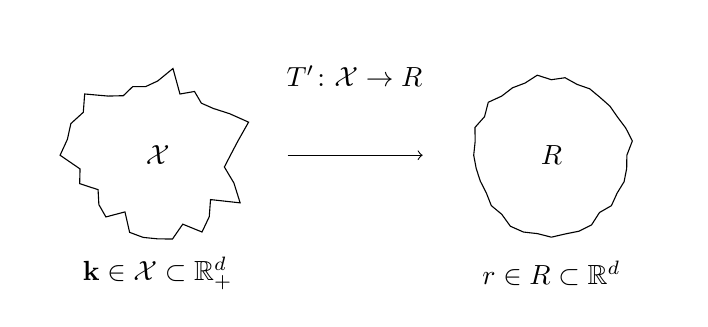
\begin{tikzpicture}
		\pgfmathsetseed{1}

		\node[inner sep=1.5cm,outer sep=0] (A) at (0,0) {$\mathcal{X}$};
		\node[inner sep=1.5cm,outer sep=0] (B) at (5,0) {$R$};

		\draw (A) \irregularcircle{1cm}{2.5mm};
		\draw (B) \irregularcircle{1cm}{0.5mm};

		\draw [->] (A) -- (B);

		\node at (2.5,1) {$T'\colon\mathcal{X}\rightarrow R$};

		\node at (0,-1.5) {$\mathbf{k}\in\mathcal{X}\subset\mathbb{R}_+^d$};
		\node at (5,-1.5) {$r\in R\subset\mathbb{R}^d$};
	\end{tikzpicture}
	\caption{Couplings between parameter space and reference when using the transport map proposal method to propose moves on parameter space.}
	\label{fig:chem_coupling}
\end{figure}

Figure~\ref{fig:chem_coupling} shows how we define a bijective map, $T'$, between parameter space $\mathcal{X}$ and a reference space $R$. In practice we cannot ensure that the approximate map $\tilde{T}'$ is uniquely invertible over the whole of $R$ and so $\tilde{T}'$ is not truly bijective. This leads to problems for our strictly positive state space, $\mathcal{X} \subset \mathbb{R}_+^d$, since proposals in $R$ do not necessarily map back on to $\mathcal{X}$. This motivates the use of a third intermediate space. When using the transport map proposal distribution, we prefix the proposal method with a T, e.g. MH-RW (RWMH) and MH-TRW, as well as PAIS-RW and PAIS-TRW.

We also consider how these algorithms perform when they are applied to the log of the reaction rates. We choose to use this log transformation since it converts our strictly positive parameter space, $\mathcal{X}$, into an intermediate space $\mathcal{Y} \subset \mathbb{R}^d$. This allows us to define $T$ between two subsets of $\mathbb{R}^d$, which means that even if $\tilde{T}$ is not uniquely invertible in some region of $R$, all possibilities are valid proposals. As before, the proposal distributions are labelled with a T for transport map and when using the intermediate space we prepend `log' to the proposal method, e.g. MH-logRW and MH-logTRW, with, PAIS-logRW and PAIS-logTRW.

\begin{figure}
	\centering
	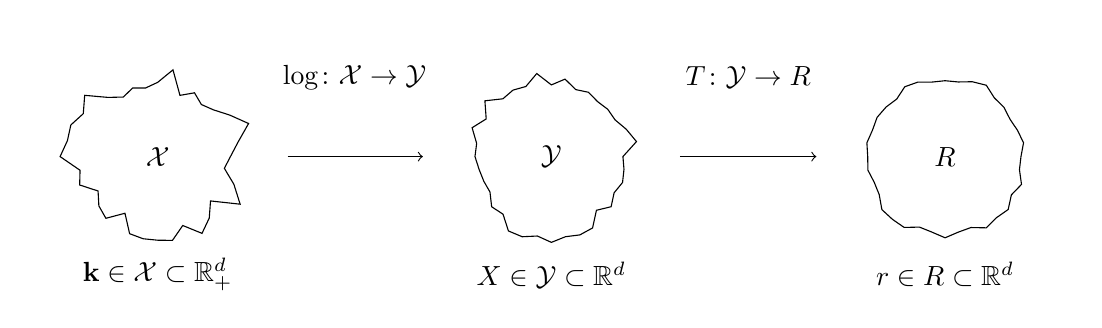
\begin{tikzpicture}
		\pgfmathsetseed{1}

		\node[inner sep=1.5cm,outer sep=0] (A) at (0,0) {$\mathcal{X}$};
		\node[inner sep=1.5cm,outer sep=0] (B) at (5,0) {$\mathcal{Y}$};
		\node[inner sep=1.5cm,outer sep=0] (C) at (10,0) {$R$};

		\draw (A) \irregularcircle{1cm}{2.5mm};
		\draw (B) \irregularcircle{1cm}{1.1mm};
		\draw (C) \irregularcircle{1cm}{0.5mm};

		\draw [->] (A) -- (B);
		\draw [->] (B) -- (C);

		\node at (2.5,1) {$\log\colon\mathcal{X}\rightarrow\mathcal{Y}$};
		\node at (7.5,1) {$T\colon\mathcal{Y}\rightarrow R$};

		\node at (0,-1.5) {$\mathbf{k}\in\mathcal{X}\subset\mathbb{R}_+^d$};
		\node at (5,-1.5) {$X\in\mathcal{Y}\subset\mathbb{R}^d$};
		\node at (10,-1.5) {$r\in R \subset\mathbb{R}^d$};
	\end{tikzpicture}
	\caption{Couplings between parameter space, an intermediate space and reference space when using the transport map proposal method to propose moves on a log space.}
	\label{fig:chem_log_coupling}
\end{figure}

Figure~\ref{fig:chem_log_coupling} displays the composition of maps when we include this intermediate space $\mathcal{Y}$. Every proposal in $R$ results in a valid proposal on $\mathcal{X}$. The inclusion of this additional map means that we must again alter our importance weight definition to reflect the pullback from $R$ through $\mathcal{Y}$. The weight is now
\[
	w_i(\theta') = \frac{\pi(\theta'|\mathbf{R},\mathbf{T})}{Q(\tilde{T}\circ\log(\theta')|\tilde{T}\circ\log(\theta^{(i-1)}))|J_{\tilde{T}\circ\log}(\theta')|},
\]
where $\theta'$ is a proposal on $\mathcal{X}$, $\theta^{(i-1)}$ is the ensemble of states from the previous iteration, and $J_{\tilde{T}\circ\log}(\theta')$ is the Jacobian of the composition of the two maps. This Jacobian is straightforward to calculate,
\[
	|J_{\tilde{T}\circ\log}(\theta')| = |J_{\tilde{T}}(\log(\theta'))||J_{\log}(\theta')|,
\]
where the first determinant is as we saw in the previous chapter, and the second is
\[
	|J_{\log}(\theta')| = \prod\limits_{i=1}^d \frac{1}{\theta'_i}.
\]

% choices made in transport map
For this problem, we continue to use monomials in each dimension in our transport map construction. We use polynomials of total order $p=4$ as the basis functions, i.e.
\[
	T_i(\theta) = \sum_{\mathbf{j}\in\mathcal{J}^{\text{TO}}_i(p)} \gamma_{i,\mathbf{j}}\psi_{\mathbf{j}}(\theta) \quad \text{where} \quad \psi_\mathbf{j}(\theta) = \prod\limits_{k=1}^i \theta_k^{j_k},
\]
and
\[
	\mathcal{J}^{\text{TO}}_i(p) = \{\mathbf{j} \in \mathbb{N}^d_0\ |\ \|\mathbf{j}\|_1 \leq p, \ \text{and}\ j_k = 0\ \forall k > i\}.
\]
Since $\mathcal{X}$ is four-dimensional, this yields a total of 125 map coefficients across the four index sets. This number can be reduced by using smaller index sets as discussed in~\cite{parno2014transport}.

% choice of resampler?
As with the mixture model in Section~\ref{sec:app_mixture}, we will use the AMR resampler with an ensemble size of $M=500$. This increase in ensemble size from Chapter~\ref{sec:PAIS} compensates for the increase in parameter dimension.

% analysis method
To measure the convergence of the sampling methods in this section, we will compare the convergence of the mean of each parameter. We approximate $\mathbb{E}(\mathbf{k})$ using 2.4 billion samples from the MH-RW algorithm.

% numerics.
\subsubsection{Convergence Analysis for the Constrained Approach to a Multiscale Chemical Reaction Model}\label{sec:chem_conv}

In this section, we demonstrate the convergence of the sample mean $\hat{\mathbf{k}}$ by approximating the relative error between the sample mean and the true mean $\mathbb{E}(\mathbf{k})$. We do this for each of the eight algorithms introduced in the previous section. Convergence is shown for the constrained approach to the multiscale system, i.e. to the posterior in Equation~\eqref{eqn:chem_QEA_posterior} with the effective degradation rate, $\hat{k}_4^{\text{CMA}}$, from Equation~\eqref{eqn:chem_CMA_rate}.

\begin{table}[!h]
\centering
\begin{tabular}{rrrrrr}
\toprule
	\multicolumn{1}{l}{Algorithm} & \multicolumn{3}{c}{MH} & \multicolumn{2}{c}{PAIS} \\ \cmidrule(lr){2-4} \cmidrule(lr){5-6}
	& & $\delta_\%$ & & $\delta_{\text{ESS}}$ & ESS \\ \midrule
	RW & & 5.5e-3 & & 1.0e-0 & 9.0e-3 \\
	TRW & & 1.2e-0 & & 4.0e-1 & 1.2e-3 \\
	logRW & & 1.7e-1 & & 1.2e-0 & 6.0e-2 \\
	logTRW & & 2.7e-2 & & 1.5e-1 & 3.5e-1 \\
\bottomrule
\end{tabular}
\caption{Optimal scaling parameters for the MH and PAIS algorithms applied to the constrained multiscale problem in Section~\ref{sec:chem_multiscale}. MH parameters optimised by acceptance rate, and PAIS parameters optimised using effective sample size.}
\label{tab:chem_multiscale_scaling}
\end{table}

The optimal scaling parameters are given in Table~\ref{tab:chem_multiscale_scaling}. We note that for MH-TRW and PAIS-TRW the scaling parameter is near to 1, particularly for MH-RW, this is what we should expect since the proposal is made on a reference space which should be near to $\mathcal{N}_d(0, \text{I})$. The same should be true for the MH-logTRW and PAIS-logTRW algorithms since these have the same target reference space, however the optimal scaling parameters here are much smaller. We see that the ESS is higher for the algorithms which sample on $\mathcal{Y}$, and we expect that convergence will be fastest for the PAIS-logTRW algorithm.

\begin{figure}[!htb]
\centering
\subfigure[Sampling algorithms on $\mathcal{X}$.]{\includegraphics[width=0.495\textwidth]{"images/CMA_L2_param_space"}}
\subfigure[Sampling algorithms on $\mathcal{Y}$.]{\includegraphics[width=0.495\textwidth]{"images/CMA_L2_log_space"}}
\caption{Convergence of the constrained multiscale example described in Section~\ref{sec:chem_multiscale}.}
\label{fig:chem_multiscale_L2}
\end{figure}

Convergence of the eight algorithms for this example is shown in Figure~\ref{fig:chem_multiscale_L2}. We first note the poor performance of the MH based algorithms, each of them taking roughly 10,000 samples to begin converging. Only the MH-TRW is at all competitive with the PAIS algorithms. During the simulation interval, the MH-TRW algorithm has not settled down to the expected $\mathcal{O}(1/\sqrt{N})$ rate which means that the estimate is still biased by the long burn-in time. As we have seen in previous examples, the burn-in time for the PAIS algorithm is negligible.

The PAIS variants with RW and TRW proposals perform similarly on both sample spaces. When sampling on $\mathcal{X}$ the transport map is not quite as efficient, largely due to the difficulties discussed in the previous section i.e. many proposals are made which do result in negative reaction rates. Sampling on $\mathcal{Y}$ leads to more comparable Monte Carlo errors, with the logTRW being apparently slightly less stable. This proposal method becomes more stable as we increase either the ensemble size, or the number of iterations between updates of the transport map, $T$. Overall we see the smallest Monte Carlo errors for a given amount of computational effort coming from the PAIS-logTRW algorithm.

\begin{figure}[!htb]
\centering
\subfigure[Reference space mapped to by $T'$.]{\includegraphics[width=0.495\textwidth]{"images/CMA_ref_space_MHTRW"}}
\subfigure[Reference space mapped to by $T\circ\log$.]{\includegraphics[width=0.495\textwidth]{"images/CMA_ref_space_MHlogTRW"}}
\caption{Reference space for the TRW and logTRW proposal distributions. Components are linked by the relation $r_i = T_i'(k_i)$ in (a) and $r_i = T_i\circ\log(k_i)$ in (b).}
\label{fig:chem_reference_spaces}
\end{figure}

We now look at the proposal distributions of the transport map accelerated algorithms. In Figure~\ref{fig:chem_reference_spaces}, we see the reference spaces found by; in (a) mapping the posterior through the map $T'$, and in (b) by mapping the posterior through $T\circ\log$. For the most part, each of these marginal distributions can be recognised as a Gaussian. However, with the exception of $\mathbb{P}(r_2,r_3)$, we would not consider them to be close to a standardised $\mathcal{N}(0, \text{I})$ distribution. Before thinking that the transport map has not helped us to find a `nicer' space on which to propose new values we should consider that the dimensions are now (1) largely uncorrelated, and (2) the variances in each dimension are much more similar than they are in Figure~\ref{fig:chem_CMA_posterior}.

Particularly in Figure~\ref{fig:chem_reference_spaces} (b) we see that $\text{var}(r_1)$ and $\text{var}(r_4)$ are much smaller than $\text{var}(r_2)$ and $\text{var}(r_3)$. To combat this we have a number of choices, we might wish to use two different scaling parameters to match these scales, which would require knowledge of the reference space before beginning sampling. We could alternatively use a proposal distribution such as in the LPAIS algorithm to adaptively learn this at each iteration. Another option is to increase the total order of our index set. For these numerics we have chosen $p=4$, but we know that we can obtain reference spaces which are closer to $\mathcal{N}_d(0, \text{I})$ by choosing a larger $p$.

\subsubsection{Comparison of the Constrained and QEA approaches}

The convergence analysis has been performed for the constrained approach to this multiscale system. We now look at the differences between the constrained and QEA posterior distributions. Recall that the approaches differed only in the form of the effective degradation rate $\hat{k}_4$,
\[
	\hat{k}_4^{\text{QEA}}(s) = \frac{k_2k_4s}{k_2+k_3} \quad \text{and} \quad \hat{k}_4^{\text{CMA}}(s) = \frac{k_2k_4s}{k_2+k_3+k_4}.
\]
This difference in the denominator causes a shift in the parameters as can be seen in Figure~\ref{fig:chem_diff}. The figure shows the difference in posteriors,
\begin{equation}\label{eqn:chem_diff}
	\text{diff}(\mu^{\text{CMA}}, \mu^{\text{QEA}}) = \pi^{\text{CMA}}(\mathbf{k}|\mathbf{R},\mathbf{T}) - \pi^{\text{QEA}}(\mathbf{k}|\mathbf{R},\mathbf{T}).
\end{equation}

\begin{figure}[htb]
\centering
\includegraphics[width=0.9\textwidth]{"images/Diff_CMA_QEA"}
\caption{Difference between the CMA and QEA posteriors as defined in Equation~\eqref{eqn:chem_diff}.}
\label{fig:chem_diff}
\end{figure}

Since the two posteriors have been approximated using an MCMC sample, there is a significant amount of noise, particularly in the tails of the distributions We can see that the differences in the marginals for $k_1, k_2,$ and $k_3$ are relatively small and the differences are largely positive. This means that the constrained approach is slightly more informative about the values of these first three parameters. However the marginal for $k_4$ varies by a significant amount and is more negative. This means that the mean estimates for $k_4$ vary by a large amount, and we should be more confident in the solution given by the QEA.

% compare solution with full data.
We now consider how we should interpret the information given by these models. The QEA assumption tells us that we cannot observe the parameters $k_2$, $k_3$ and $k_4$ independently from the reduced data set, but we can observe the quantity $\hat{k}_4^{\text{QEA}} = k_2k_4/(k_2+k_3)$. Similarly, the constrained approach tells us that we are able to observe the quantity $\hat{k}_4^{\text{CMA}} = k_2k_4/(k_2+k_3+k_4)$. To validate our inferences on $k_2$, $k_3$ and $k_4$ we would like to discover which model is most informative about these parameters, and which model gives us results which are most similar to what we can obtain from the full model.

A conventional way to compare two models under a Bayesian framework is to calculate the Bayes factors~\cite{chen2012monte}. The Bayes factor, $B_{1,2}$, between two models, $\mathcal{M}_1$ and $\mathcal{M}_2$, can be interpreted as a ratio of the normalisation constants of the posterior distributions given each model,
\[
	B_{1,2} = \frac{\mathbb{P}(D|\mathcal{M}_1)}{\mathbb{P}(D|\mathcal{M}_2)}, \quad \text{where} \quad \mathbb{P}(D|\mathcal{M}_k) = \int_\mathcal{X} \mathbb{P}(D|\theta_k,\mathcal{M}_k)\mathbb{P}(\theta_k|\mathcal{M}_k) \, \text{d}\theta_k.
\]
Under the PAIS framework, it is straightforward to calculate these factors using the Monte Carlo estimator for the normalisation constants. From~\cite{robert2013monte} these normalisation constants take the form
\[
	Z_k \approx \hat{Z}_k\frac{1}{NM}\sum_{i=1}^N\sum_{j=1}^M w_j^{(i)}(\mathcal{M}_k),
\]
where $w_j^{(i)}(\mathcal{M}_k)$ is the weight under model $\mathcal{M}_k$ corresponding to the $j$-th ensemble member on the $i$-th iteration. Hence, $B_{1,2} \approx \hat{Z}_1/\hat{Z}_2$. We can compare more than two models in this way by selecting the model with the largest marginal distribution as the best model.

We now label the constrained model as $\mathcal{M}_1$, the model arising from the QEA as $\mathcal{M}_2$, and the full data model as $\mathcal{M}_0$. Under $\mathcal{M}_1$, the parameter $\theta_1 = (k_1, \hat{k}_4^{\text{CMA}})^\top$, and under $\mathcal{M}_2$, the parameter $\theta_2 = (k_1, \hat{k}_4^{\text{QEA}})^\top$. The full model $\mathcal{M}_0$ observes all four parameters $\theta_0 = (k_1, k_2, k_3, k_4)^\top$. The marginal densities for the data, evaluated at the observed data, given the models are displayed in Table~\ref{tab:chem_Bayes_marginals}.

\begin{table}[!htb]
\centering
\begin{tabular}{rr}
	\toprule
	$k$ & \quad $\mathbb{P}(D = (\mathbf{R},\mathbf{T})^\top|\mathcal{M}_k)$ \\ \cmidrule(lr){1-2}
	0 & 6.8e-3 \\
	1 & 3.2e-3 \\
	2 & 1.7e-3 \\ \bottomrule
\end{tabular}
\caption{Marginal distributions for the data $(\mathbf{R},\mathbf{T})^\top$ for each model considered in Section~\ref{sec:multiscale_posterior}.}
\label{tab:chem_Bayes_marginals}
\end{table}

Computing the Bayes factors from Table~\ref{tab:chem_Bayes_marginals} we see that we should of course prefer the model in which we observe all reactions perfectly, however this model is not significantly better than the CMA model ($B_{0,1} = 2.09 < 3.2$, ~\cite{kass1995bayes}). Again the constrained model is not substantially more attractive than the QEA model when we consider the Bayes factor $B_{1,2} = 1.96 < 3.2$. The Bayes factor $B_{0,2} = 4.1 > 3.2$ does tell us that we should significantly prefer the full model to the QEA model. These Bayes factors present a weak argument that that the constrained model provides us with a better description of the data than the QEA model. We can also present this information graphically, which might provide us with a greater justification for preferring the constrained model.

\begin{figure}[!htb]
\centering
\subfigure[Marginal for $\hat{k}_4^{\text{QEA}}$.]{\includegraphics[width=0.495\textwidth]{"images/QEA_approx_marginal"}}
\subfigure[Marginal for $\hat{k}_4^{\text{CMA}}$.]{\includegraphics[width=0.495\textwidth]{"images/CMA_approx_marginal"}}
\caption{Comparison of the approximate marginal densities for the `observable parameter' $\hat{k}_4$ under models $\mathcal{M}_1$ and $\mathcal{M}_2$. Marginals for these two parameters are approximated using samples which have been produced by targeting the three densities $\pi_i = \mathbb{P}(\theta_i|D,\mathcal{M}_i)$ for $i = 0, 1, 2$.}
\label{fig:chem_model_comp}
\end{figure}

Figure~\ref{fig:chem_model_comp} displays the marginal distributions for the parameters $\hat{k}_4^{\text{QEA}}$ and $\hat{k}_4^{\text{CMA}}$. For each of these two observable parameters we obtain approximations for three marginal distributions, $\pi_i(\cdot|D, \mathcal{M}_i)$, $i = 0, 1, 2$. Each of these approximations has been produced by marginalising a sample drawn from the full posterior $\pi_i(\mathbf{k}|D, \mathcal{M}_i)$ defined in terms of the respective model $\mathcal{M}_i$. In other words, to calculate $\hat{\pi}_1(\hat{k}_4^{\text{QEA}}|D)$, we first draw a sample using the PAIS algorithm targeting the posterior density $\pi_1(\mathbf{k}|D,\mathcal{M}_1)$. We then calculate $\theta^{(j)} = k_2^{(j)}k_4^{(j)}/(k_2^{(j)}+k_3^{(j)})$ for each sample produced. Finally we produce a histogram from this sample $\theta^{(j)}$.

The first thing to note is that in subfigure (a) when we approximate the marginals for $\hat{k}_4^{\text{QEA}}$ the density $\hat{\pi}_2(\cdot|D,\mathcal{M}_2)$ is much more peaked than $\hat{\pi}_1(\cdot|D,\mathcal{M}_1)$. As we might expect the same is true in reverse in subfigure (b). What is interesting here is that for both parameters, the marginal distribution which assumes $\mathcal{M}_2$ assigns a small density value to the true value of the parameter, while the marginals which assume $\mathcal{M}_1$ assign a relatively high density to the truth. We also draw attention to the similarities between the constrained model and the full data model. In subfigure (a) these two marginals are peaked around a similar value, and in subfigure (b) the full data and constrained models almost exactly coincide. This supports the hypothesis that the constrained approach provides a more accurate approximation to the dynamics of the full system.

\subsection{Gene Regulatory Networks}\label{sec:grn}
In this example, we look at a model of a gene regulatory network (GRN) mechanism used by a particular cell to regulate the amount of a protein, $P$, present. In this model, we again have reactions occurring at particular rates, $k$, between four different species. Here there is a special species, $G$, representing the gene responsible for building the protein, of which there is only one at a time, and this species can either be turned on or off. When the gene is off we denote it as $G'$.
\begin{align}
	P+P \xleftrightarrows[k_2]{k_1} D \quad & \quad G+D \xleftrightarrows[k_4]{k_3} G' \nonumber\\
	G \xrightarrow{k_5} G+M \quad & \quad M\xrightarrow{k_6} M+P  \label{eqn:GRN_reactions} \\
	P \xrightarrow{k_7} \emptyset \quad & \quad M \xrightarrow{k_8} \emptyset \nonumber
\end{align}
The eight reactions are given in Equation~\eqref{eqn:GRN_reactions}. In addition to the gene, $G$, and protein, $P$, the system also involves molecules of mRNA, $M$, and dimers, $D$, which are two proteins joined together.

In this example, similar to those found in ***citations***, protein is created by a molecules of mRNA at a rate $k_6$. The amount of protein in the cell is then governed by the rate of decay of $P$, and the number of mRNA molecules in the cell creating $P$. In turn the number of mRNA molecules is controlled by its own decay rate and whether or not the gene $G$, which produces the mRNA is active. The gene can be turned on and off depending on how many dimers are present in the system, which is related to how many protein molecules there are. This completes a feedback cycle whereby if the protein population gets too high then the gene will turn off and the rate of new protein formation will decrease, causing the level to drop and the gene to turn back on.

\begin{figure}
	\centering
	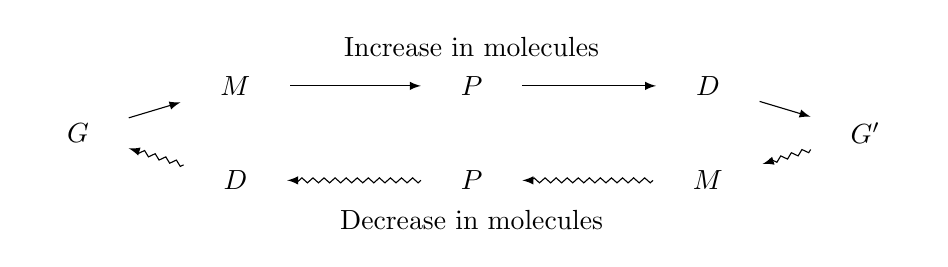
\begin{tikzpicture}

		\node at (0, 1.1) {Increase in molecules};

		\node[inner sep=.5cm] (AA) at (-3,.6) {$M$};
		\node[inner sep=.5cm] (BB) at (0,.6) {$P$};
		\node[inner sep=.5cm] (CC) at (3,.6) {$D$};
		\node[inner sep=.5cm] (DD) at (5,0) {$G'$};

		\node at (0, -1.1) {Decrease in molecules};

		\node[inner sep=.5cm] (EE) at (3,-.6) {$M$};
		\node[inner sep=.5cm] (FF) at (0,-.6) {$P$};
		\node[inner sep=.5cm] (GG) at (-3,-.6) {$D$};
		\node[inner sep=.5cm] (HH) at (-5,0) {$G$};

		\draw [arrows={-latex}] (HH) -- (AA);
		\draw [arrows={-latex}] (AA) -- (BB);
		\draw [arrows={-latex}] (BB) -- (CC);
		\draw [arrows={-latex}] (CC) -- (DD);
		\draw [arrows={-latex},decorate, decoration={zigzag, segment length=4, amplitude=.9,post=lineto, post length=2pt}] (DD) -- (EE);
		\draw [arrows={-latex},decorate, decoration={zigzag, segment length=4, amplitude=.9,post=lineto, post length=2pt}] (EE) -- (FF);
		\draw [arrows={-latex},decorate, decoration={zigzag, segment length=4, amplitude=.9,post=lineto, post length=2pt}] (FF) -- (GG);
		\draw [arrows={-latex},decorate, decoration={zigzag, segment length=4, amplitude=.9,post=lineto, post length=2pt}] (GG) -- (HH);
	\end{tikzpicture}
	\caption{Diagram of the effects of molecule populations in a gene regulatory network.}
	\label{fig:grn_cycle}
\end{figure}

As in Section~\ref{sec:chem_multiscale} we use the constrained multiscale approach to model the system. The formulation here is slightly more complex. We define a fast subsystem which acts on the fast variables $\mathcal{F} = [P, D, G]$ and incorporates reactions $R_1$-$R_4$, 90\% of reactions which occur in a particular time frame are one of these four reactions.
\[
	\text{Fast subsystem:} \quad P+P\xleftrightarrows[k_2]{k_1} D, \quad G+D\xleftrightarrows[k_4]{k_3} G'.
\]
We also define the slow variables, $T = P+2D+2(1-G)$ and $M$ which are held constant by these fast reactions.

When we observe a cell, we cannot distinguish between the fast species and so don't know which of the first four reactions are happening. Due to this, we observe how many of reactions $R_5$-$R_8$ occur for each combination of the two slow variables $\mathcal{S} = [T, M]$. Since we don't observe $P$ and $G$ for every reaction, the propensities must be altered to take this into account,
\begin{align}
	\hat{\alpha}_5 = k_5\mathbb{E}[G|T],\quad&\quad \alpha_6 = k_6M, \notag\\
	\hat{\alpha}_7 = k_7\mathbb{E}[P|T], \quad&\quad \alpha_8 = k_8M.\label{eqn:grn_propensities}
\end{align}
To calculate these expectations, we note that the fast subsystem is a deficiency zero system ***citations***, and is also reversible. i.e. The system has four complexes, 
\[
	C_1 = P+P, \quad C_2 = D, \quad C_3 = G+D \quad \text{and} \quad  C_4 = G',
\]
there are two linkage classes (or two sets of reversible reactions), and the space spanned by the stoichiometries is two dimensional,
\[
	\text{span}\left\{\pm[-2, 1, 0, 0]^\top, \pm[0, -1, 0, -1]^\top\right\},
\]
hence the deficiency is $d = 4 - 2 - 2 = 0$. This means that the conditional probabilities have the closed form equation,
\[
	\mathbb{P}[\mathcal{F}|T] \propto \text{Poisson}(P_T;\bar{p})\text{Poisson}(D_T;\bar{d})\text{Poisson}(G_T;\bar{g})\text{Poisson}(1-G_T;1-\bar{g}),
\]
from which we can calculate the expected values of $P$, $D$, and $G$. The fast variables $P_T$, $D_T$ and $G_T$ are constrained to the line defined by $T=P+2D+2(1-G)=t$. The concentrations $\bar{p}$, $\bar{d}$ and $\bar{g}$, must be calculated as the solution to the nonlinear system produced by examining the steady state behaviour of the fast subsystem,
\begin{align}
	T &= p + 2d + 2(1-g), \notag\\
	\frac{\text{d}p}{\text{d}t} &= -2k_1p^2+2k_2d = 0, \notag\\
	\frac{\text{d}d}{\text{d}t} &= k_1p^2 - k_2d - k_3gd + k_4(1-g) = 0, \notag\\
	\frac{\text{d}g}{\text{d}t} &= -k_3gd + k_4(1-g) = 0, \label{eqn:grn_nonlinear_system}
\end{align}
subject to $p \in [0, T]$.

With these effective propensities, given in Equation~\eqref{eqn:grn_propensities}, we can calculate the posterior distribution as given in Equation~\eqref{eqn:chem_posterior}, again assigning Gamma priors to the eight reaction rates. We note that the reaction rates for the fast variables do not appear in the posterior density explicitly which only uses the propensities $\alpha_5$-$\alpha_8$, however they appear through the solution to the nonlinear system in Equation~\eqref{eqn:grn_nonlinear_system}.

\subsubsection{Target Distribution}

As in the previous chemical system example we use the target distribution as defined in Equation~\eqref{eqn:chem_posterior}. The application here is slightly more involved as discussed previously in Section~\ref{sec:grn}. We have an eight dimensional parameter space, with one reaction rate corresponding to one of eight reactions. The first four reactions, $R_1$-$R_4$, are combined into a fast subsystem for which we do not observe the time or identifier for which reaction has fired. We instead use the constrained multiscale approach to approximate what has happened in this subsystem between occurrences of the slow reactions firing (reactions $R_5$-$R_8$). For this reason, we apply the form in Equation~\eqref{eqn:chem_posterior} to reactions $R_5$-$R_8$, and allow the rates for reactions $R_1$-$R_4$ to implicitly influence the posterior density through the effective propensities, $\hat{\alpha}_5$ and $\hat{\alpha}_7$.

As we mentioned earlier, for this problem we only consider the CMA's approximation to the system dynamics.

The priors for this problem were chosen to be fairly uninformative with respect to the likelihood function for each reaction rate. A list of the hyper-parameters corresponding to each Gamma prior can be found in Table~\ref{tab:grn_priors}.

\begin{table}[!h]
\centering
\begin{tabular}{|l|R{1.8em}|R{1.8em}|R{1.8em}|R{1.8em}|R{1.8em}|R{1.8em}|R{1.8em}|R{1.8em}|}
	\hline
	Dimension $i$ & 1 & 2& 3& 4 & 5 & 6 & 7 & 8 \\ \hline
	$\alpha_i$ & 2 & 100 & 100 & 3 & 3 & 3 & 2 & 2\\ \hline
	$\beta_i$ &50 & 0.02 & 1 & 1 & 0.6 & 1 & 50 & 50 \\ \hline
\end{tabular}
\caption{Hyper parameters for the Gamma priors on each of the reaction rates in the GRN example in Section~\ref{sec:grn}.}
\label{tab:grn_priors}
\end{table}

\begin{figure}[htb]
\centering
\makebox[\textwidth][c]{\includegraphics[width=1.2\textwidth]{"images/GRN_posterior"}}%
\caption{Marginal densities of the posterior distribution for the GRN example in Section~\ref{sec:grn}.}
\label{fig:GRN_posterior}
\end{figure}

The one- and two-dimensional marginal distributions for the full posterior distribution are displayed in Figure~\ref{fig:GRN_posterior}. The posterior does not contain many interesting correlation structures, however several dimensions have leptokurtic tails which are difficult for the standard PAIS algorithm to sample from. The marginal densities also vary over very different scales, which might require us to use a variant of the LPAIS algorithm.

\subsubsection{Implementation}

%% proposal methods
%For the posterior distribution in \eqref{eqn:chem_QEA_posterior}, we consider several proposal methods. First we implement both the PAIS and MH algorithms with a Gaussian proposal distribution. In the case of the PAIS algorithm, this is a Gaussian mixture proposal distribution. The proposal distribution uses a covariance matrix which has been constructed using the sample covariance of a sample produced using a standard RWMH algorithm. We also compare the PAIS and MH algorithms when using a transport map proposal distribution. This proposal method was discussed in detail in Chapter~\ref{sec:TransportPAIS}.
%
%
%Figure~\ref{fig:chem_coupling} shows how we define a bijective map, $T'$, between parameter space $\mathcal{X}$ and a reference space $R$. In practice we cannot ensure that the approximate map $\tilde{T}'$ is uniquely invertible over the whole of $R$ and so $\tilde{T}'$ is not truly bijective. This leads to problems for our strictly positive state space, $\mathcal{X} \subset \mathbb{R}_+^d$, since proposals in $R$ do not necessarily map back on to $\mathcal{X}$. This motivates the use of a third intermediate space. When using the transport map proposal distribution, we prefix the proposal method with a T, e.g. MH-RW (RWMH) and MH-TRW, as well as PAIS-RW and PAIS-TRW.
%
%We also consider how these algorithms perform when they are applied to the log of the reaction rates. We choose to use this log transformation since it converts our strictly positive parameter space, $\mathcal{X}$, into an intermediate space $\mathcal{Y} \subset \mathbb{R}^d$. This allows us to define $T$ between two subsets of $\mathbb{R}^d$, which means that even if $\tilde{T}$ is not uniquely invertible in some region of $R$, all possibilities are valid proposals. As before, the proposal distributions are labelled with a T for transport map and when using the intermediate space we prepend `log' to the proposal method, e.g. MH-logRW and MH-logTRW, with, PAIS-logRW and PAIS-logTRW.
We apply the eight RW and logRW proposal distributions, with and without transport map acceleration, which were discussed in Section~\ref{sec:chem_multiscale} to this posterior. Again the intermediate log space is required so that our transport map is a function $T\colon\mathbb{R}^d\rightarrow\mathbb{R}^d$, rather than a map from $\mathbb{R}_+^d$ to $\mathbb{R}^d$.

%% choices made in transport map
%For this problem, we continue to use monomials in each dimension in our transport map construction. We use polynomials of total order $p=4$ as the basis functions, i.e.
%\[
%	T_i(\theta) = \sum_{\mathbf{j}\in\mathcal{J}^{\text{TO}}_i(p)} \gamma_{i,\mathbf{j}}\psi_{\mathbf{j}}(\theta) \quad \text{where} \quad \psi_\mathbf{j}(\theta) = \prod\limits_{k=1}^i \theta_k^{j_k},
%\]
%and
%\[
%	\mathcal{J}^{\text{TO}}_i(p) = \{\mathbf{j} \in \mathbb{N}^d_0\ |\ \|\mathbf{j}\|_1 \leq p, \ \text{and}\ j_k = 0\ \forall k > i\}.
%\]
%Since $\mathcal{X}$ is four-dimensional, this yeilds a total of 125 map coefficients across the four index sets. This number can be reduced by using smaller index sets as discussed in~\cite{parno2014transport}.
The transport map setup has not changed from the previous example. However, due to the scaling of the weight we have had to be more careful about which samples we use to build our map. We require that the objective function $C(T)$, from Equation~\eqref{eqn:TPAIS_objective} is convex, which requires that the second derivative, given in Equation~\eqref{eqn:TPAIS_hessian}, is positive definite. This positive definite property depends on all weights in our sample being strictly positive, which is not always possible on a computer. For this reason we filter out any samples from the optimisation problem where the weight is a numeric zero. This does not affect the validity of the map since a weight zero would not contribute to the expectation, and we do not require (and could not enforce) an exact map.

In all eight algorithms we adapt the proposal variances during the burn-in phase of the algorithms to avoid behaviour like that seen in Example~\ref{sec:ex_W1} where we needed a huge ensemble size to approximate the posterior with our mixture of isotropic Gaussian kernels.

%% choice of resampler?
%As with the mixture model in Section~\ref{sec:app_mixture}, we will use the AMR resampler with an ensemble size of $M=500$. This increase in ensemble size from Chapter~\ref{sec:PAIS} compensates for the increase in parameter dimension.
We again use the AMR resampler, this time with an ensemble size of $M=2500$. The increase in ensemble size again compensates for the increase in dimension (from four to eight parameters.)

%% analysis method
%To measure the convergence of the sampling methods in this section, we will compare the convergence of the mean of each parameter. We approximate $\mathbb{E}(\mathbf{k})$ using 2.4 billion samples from the MH-RW algorithm.
As in the previous chemical reaction example, we measure convergence of the algorithms only through the convergence of the mean, for computational ease. We use the sample Mahalanobis distance, with `true' covariance and `true' mean built from a sample of size 2.4 billion using the MH-RW algorithm.

\subsubsection{Convergence results}

The scaling parameter selection is done by optimising the acceptance rate for the MH algorithms, and optimising the effective sample size for the PAIS algorithms. The optimal parameters are given in Table~\ref{tab:grn_scaling_parameters}.

\begin{table}[!h]
	\centering
	\begin{tabular}{lrrrrrrrr}
	\toprule
		 & \multicolumn{4}{c}{MH} & \multicolumn{4}{c}{PAIS} \\ \cmidrule(lr){2-5} \cmidrule(lr){6-9}
		& RW & logRW & TRW & log-TRW & RW & logRW & TRW & log-TRW \\ \midrule
		$\beta_{\%}^*$	 	& 1.0e-1 & 3.9e-1 & 1.0e-0 &6.0e-1 & - & - & - & - \\
		$\beta_{\text{ESS}}^*$	& - 	        & -           & -            & -            & 1.0e-0 & 1.3e-0 & 8.0e-1 & 5.0e-1 \\
		ESS/$M$		 		& - 	        & -           & -            & -            & 3.5e-4 & 4.7e-2 & 4.8e-2 & 1.6e-1  \\
	\bottomrule
	\end{tabular}
	\caption{Scaling parameters for the sampling algorithms applied to the GRN example in Section~\ref{sec:grn}.}
	\label{tab:grn_scaling_parameters}
\end{table}

From the effective sample sizes shown in Table~\ref{tab:grn_scaling_parameters} we can see the improvement to the efficiency of the algorithm both by proposing on the log space, and by transforming the parameter space into something closer to Gaussian.

Due to the numerical cost of calculating the full relative $L^2$ errors for this posterior, we quantify the convergence speeds of these algorithms using the sample Mahalanobis distance between the sample mean and the `true' mean. This convergence analysis is shown in Figure~\ref{fig:grn_L2}.

\begin{figure}[!htb]
\centering
\subfigure[Sampling algorithms on $\mathcal{X}$.]{\includegraphics[width=0.495\textwidth]{"images/GRN_convergence"}}
\subfigure[Sampling algorithms on $\mathcal{Y}$.]{\includegraphics[width=0.495\textwidth]{"images/GRN_convergence_log"}}
\caption{Convergence of the GRN example described in Section~\ref{sec:grn}.}
\label{fig:grn_L2}
\end{figure}

The first thing to note is that the first PAIS measurement happens after 2500 samples, whereas the first MH measurement occurs after 50 samples. This is due to the much larger ensemble size required to sample in higher dimensions. We believe that an ensemble size of 2500 is over-cautious in this example and we could have used a smaller ensemble size. We also think that the required ensemble size to sample from these posteriors is reduced by the use of the transport map. This is due to the way the tail behaviour is improved by the transformation.

The second obvious feature of these convergence plots is that the PAIS algorithms outperform the MH algorithms by a large margin - roughly a reduction of two orders of magnitude in the relative error over the same number of samples. A less positive result is that for this example the PAIS-TRW algorithm has found a map which has prevented further convergence of the mean. This is likely because the one dimension of the transport map is sending proposals onto the negative real line and so all samples are being assigned a zero weight. This is behaviour which was anticipated, and it is always suggested that the transport map is constructed as a map $T\colon\mathbb{R}^d\rightarrow\mathbb{R}^d$ rather than $T\colon\mathcal{X}\rightarrow\mathbb{R}^d$ where $\mathcal{X}\subset\mathbb{R}^d$. Despite the large increase in the effective sample size observed between the PAIS-logRW and PAIS-logTRW algorithms, this improvement is  converted into an estimate which is twice as accurate after 1 million samples.

A similar pattern is seen in the MH algorithms, where the MH-TRW performs the worst, and the MH-logTRW algorithm performs the best, although only marginally.

\bibliographystyle{siam}
\bibliography{refs}
\end{document}
